% Full paper draft — compile from docs/: pdflatex QCE_Router_Paper_main.tex
%
% OVERLEAF (one .tex + bibliography):
%   1. Upload this file (or your merged single .tex) AND QCE_Router_Paper.bib in the same folder.
%   2. Menu -> Main document -> this file.
%   3. Preamble MUST include: \usepackage[round,authoryear]{natbib}
%   4. Before \end{document}, AFTER main text / BEFORE appendix, keep:
%        \bibliographystyle{plainnat}
%        \bibliography{QCE_Router_Paper}
%   5. In body use \citep{key} or \citet{key} (keys must match QCE_Router_Paper.bib).
%   6. Recompile; if cites show "?", click Recompile again (Overleaf runs BibTeX automatically).
%
\documentclass[11pt]{article}
\usepackage{amsmath,amssymb}
\usepackage{booktabs}
\usepackage{multirow}
\usepackage{graphicx}
\usepackage[round,authoryear]{natbib}  % load before hyperref
\usepackage{hyperref}
\usepackage{algorithm}
\usepackage{algpseudocode}
\usepackage{listings}
\usepackage{tikz}
\usetikzlibrary{arrows.meta,positioning,fit,calc}
\usepackage[most]{tcolorbox}
\usepackage{caption}
\usepackage{ragged2e}
% Helps two-column floats (prompt figure*, GAIA figure*) place correctly.
\usepackage{dblfloatfix}
\lstset{
  basicstyle=\ttfamily\scriptsize,
  breaklines=true,
  columns=fullflexible,
  keepspaces=true,
  showstringspaces=false,
}
\lstdefinestyle{promptsuite}{
  basicstyle=\ttfamily\scriptsize,
  breaklines=true,
  breakatwhitespace=false,
  columns=fullflexible,
  keepspaces=true,
  showstringspaces=false,
  tabsize=2,
  frame=none,
  aboveskip=0pt,
  belowskip=0pt,
  inputencoding=utf8,
  extendedchars=true,
}

% Figure search paths (compile from repo root or upload same tree on Overleaf).
\graphicspath{{figures/}{results/reports/figures/}{results/reports/router/test/}{results/reports/router/val/}{results/reports/analysis/}}

\title{Adaptive Agent Routing: Plan-Structure-Guided Cost-Soft Selection for LLM Agent Strategies}
\author{Anonymous Authors}
\date{}

\begin{document}
\maketitle

% Abstract — problem → gap → method → results (research-story order)
\begin{abstract}
Deploying large language model (LLM) agents requires selecting among heterogeneous agent
strategies, including direct prompting, chain-of-thought reasoning, tool-augmented ReAct, and
multi-agent coordination.
Because no single strategy is optimal across queries, effective deployment depends on routing
queries to appropriate strategies before execution.
Existing routing approaches primarily rely on semantic query representations and hard
winner-take-all supervision, which may overlook procedural requirements and discard information
when multiple strategies succeed at different costs.

We propose \textbf{Adaptive Agent Routing (AAR)}, a pre-inference routing framework that combines
planner-derived procedural complexity with semantic query representations.
AAR first estimates query complexity from an LLM-generated procedure directed acyclic graph
(DAG), summarized into a five-dimensional complexity vector.
This signal is fused with semantic embeddings to form a complexity--semantic routing
representation.
To learn routing policies, AAR employs \textbf{cost-soft supervision}, which distributes
training mass across successful strategies according to execution cost rather than enforcing a
single hard target.

Experiments on a held-out routing benchmark ($n{=}100$ test; $\lambda{=}25$) show that
\textbf{cost-soft supervision} substantially reduces utility regret (agent regret
$0.361\to 0.192$; executed exact match 63\%$\to$82\%).
The lowest total regret ($0.198$) is achieved when cost-soft training is combined with the
complexity--semantic representation, outperforming embedding-only, complexity-only, and
heuristic-plus-embedding baselines.
Representation ablations indicate that procedural complexity alone is insufficient for routing
but provides complementary information when combined with semantic features.
Under transfer on executed benchmark workloads ($N{=}965$), AAR attains competitive performance
(48.1\% pooled exact match vs.\ 50.3\% for a heuristic baseline); gains are less consistent
than on the routing benchmark, where oracle multi-strategy supervision aligns with the routing
objective.
\end{abstract}

% Section 1: Introduction — Adaptive Agent Routing (AAR)
\section{Introduction}
\label{sec:intro}

Large language models (LLMs) increasingly power agentic systems that perform multi-step
reasoning, retrieval, tool use, and coordinated execution.
As these agentic systems mature, they expose multiple \textbf{agent strategies}---raw direct
prompting, chain-of-thought (CoT), ReAct-style tool use, and multi-agent coordination---each
with distinct performance and inference costs for the same query.

Despite this growing diversity, deployed agentic systems typically apply a \textbf{single fixed
agent strategy} to every query.
Query demands are not uniform: some instances are solvable with lightweight prompting, while
others require multi-step reasoning, retrieval, or multi-agent orchestration.
A static \textbf{routing policy} can therefore misalign execution cost with task requirements and
weaken the \textbf{performance--cost trade-off} across heterogeneous workloads.
On five executed benchmark workloads---GAIA~\citep{mialon2023gaia}, HotpotQA~\citep{yang2018hotpotqa},
MuSiQue~\citep{trivedi2022musique}, MMLU-Pro~\citep{wang2024mmlupro}, and MATH~\citep{hendrycks2021math}
($N{=}965$)---the best fixed strategy is not universal: ReAct~\citep{yao2023react} attains the
highest exact match on four suites while chain-of-thought~\citep{wei2022cot} leads on MATH
(Figure~\ref{fig:fixed-strategy-em}).

\begin{figure}[t]
  \centering
  \footnotesize
  \setlength{\tabcolsep}{3pt}
  \caption{Exact match (\%) when each agent strategy is run in isolation ($n{=}965$ pooled).}
  \label{fig:fixed-strategy-em}
  \begin{tabular}{@{}lrrrrr@{}}
    \toprule
    Workload & raw & cot & react & multiagent & Best fixed \\
    \midrule
    GAIA & 4.2 & 6.1 & \textbf{26.1} & 13.3 & react \\
    HotpotQA & 39.5 & 36.5 & \textbf{69.0} & 32.0 & react \\
    MuSiQue & 2.5 & 2.5 & \textbf{36.5} & 25.5 & react \\
    MMLU-Pro & 48.5 & 53.0 & \textbf{59.0} & 46.5 & react \\
    MATH & 31.0 & \textbf{69.5} & 63.0 & 56.0 & cot \\
    \bottomrule
  \end{tabular}
\end{figure}

Prior routing methods demonstrate that adaptive selection can improve efficiency.
However, much of this literature addresses \textbf{model routing}---selecting among strong and
weak LLMs or API tiers~\citep{ong2025routellm,chen2024routerdc}---rather than routing among
heterogeneous \textbf{agent strategies}.
Routing signals in related work are often based on semantic query representations,
query--candidate interaction graphs, or latent difficulty
estimates~\citep{feng2025graphrouter,su2026daao}, and seldom encode the anticipated execution
procedure that a query implies.

This matters because semantically similar queries can require substantially different execution
procedures due to differences in dependency structure, reasoning depth, external information
requirements, or coordination demands.
Consequently, effective routing requires signals that capture not only what a query is about,
but also how it is likely to be solved.
Agent strategies differ primarily in the kinds of procedures they execute; therefore routing
decisions should depend not only on query content but also on anticipated procedural complexity.
When supervised routing uses a single winning label, \textbf{hard supervision} also discards
information when multiple agent strategies succeed at different costs.
Unlike prior routers that rely primarily on flat query embeddings, we propose
\textbf{Adaptive Agent Routing (AAR)}, which incorporates \textbf{query complexity}
estimated from planner-derived procedural structures as an explicit signal for pre-inference
strategy selection over
$\mathcal{A}=\{\texttt{raw},\texttt{cot},\texttt{react},\texttt{multiagent}\}$.
AAR further trains with \textbf{cost-soft supervision} that preserves information from multiple
successful agent strategies rather than enforcing a single winner.
\textbf{Procedural complexity} provides pre-execution information about anticipated reasoning,
retrieval, tool use, and coordination demands that is unavailable from semantic representations
alone.
The routing objective is formalized in \S\ref{sec:problem}; the Query Complexity Estimator (QCE)
and routing policy are described in \S\ref{sec:method}.

\paragraph{Research question.}
\textbf{RQ1:} Can planner-derived estimates of query complexity improve pre-inference
agent-strategy routing under a performance--cost objective?

\paragraph{Our solution.}
To answer RQ1, we propose \textbf{Adaptive Agent Routing (AAR)}, a pre-inference
agent-strategy routing framework built on three steps:
\textbf{(i)}~the \textbf{Query Complexity Estimator (QCE)} estimates query complexity from
planner-derived procedural structures;
\textbf{(ii)}~query complexity is \textbf{fused} with a semantic query embedding to form the
complexity--semantic routing representation fed to the router;
\textbf{(iii)}~a \textbf{routing policy} is learned from \textbf{cost-soft supervision} over
empirical agent outcomes, retaining mass on cheaper successful strategies instead of collapsing
to one hard label.
At deployment, only the selected strategy in $\mathcal{A}$ executes, preserving the efficiency of
single-strategy serving.

\paragraph{Why it matters.}
Query complexity provides information about anticipated execution requirements that is
unavailable from semantic representations alone.
Incorporating such signals into routing decisions enables strategy selection based on expected
procedural demands rather than query content alone.
Cost-soft supervision further aligns training with deployment utility when multiple agent
strategies in $\mathcal{A}$ are correct at different costs.
Deployed agentic systems can thereby improve the cost-aware trade-off under single-strategy
execution without running all four agent strategies on every query.

\paragraph{Contributions.}
Our contributions are:
\begin{enumerate}
  \item We propose \textbf{cost-soft supervision}, which preserves signal from all strategies
    that succeed at different cost points rather than enforcing a single hard winning label.
  \item We introduce a \textbf{complexity--semantic routing representation} that fuses
    planner-derived procedural complexity with semantic embeddings; ablations show that
    complexity provides complementary routing information when combined with embeddings, not
    when used in isolation.
  \item We evaluate AAR on a stratified routing benchmark and on transfer workloads---including
    representation and supervision ablations---showing that cost-soft supervision contributes
    the largest regret reduction and that the best configuration combines cost-soft training
    with complexity--semantic features (\S\ref{sec:experiments}).
\end{enumerate}

% Section 2: Problem Formulation (features in Sec. 3; evaluation in Sec. 4)
\section{Problem Formulation}
\label{sec:problem}

We study \textbf{pre-inference agent-strategy routing} for \textbf{Adaptive Agent Routing
(AAR)}: given a query, select one \textbf{agent strategy} to execute before any strategy runs,
using only pre-execution features.

\subsection{Pre-Inference Agent-Strategy Routing}
\label{sec:goal}

Given a query $q$, the objective is to select an agent strategy from a fixed pool
\begin{equation}
  \mathcal{A}=\{a_1,\ldots,a_4\}=\{\texttt{raw},\texttt{cot},\texttt{react},\texttt{multiagent}\},
  \label{eq:strategy-set}
\end{equation}
before any agent strategy is executed.
Each member of $\mathcal{A}$ is a full execution policy---direct prompting (\texttt{raw}),
chain-of-thought (\texttt{cot}), ReAct-style tool use (\texttt{react}), or multi-agent
coordination (\texttt{multiagent})---not merely a reasoning style.

For each query $q$ and strategy $a\in\mathcal{A}$, executing $a$ produces an answer
$\hat{y}_a(q)$, an exact-match outcome $r_a(q)\in\{0,1\}$, and an execution cost
$c_a(q)\ge 0$.
Outcome $r_a(q)=1$ indicates exact-match success with a valid answer; $r_a(q)=0$ otherwise.
A \textbf{routing policy} selects $\hat{a}(q)\in\mathcal{A}$ using only information available
prior to execution, and the system returns
\begin{equation}
  \hat{y}(q)=\hat{y}_{\hat{a}(q)}(q).
  \label{eq:output}
\end{equation}
At deployment, exactly one agent strategy is selected and executed; unlike ensemble or fusion
approaches, no multiple strategies run on the same query.

Each agent strategy induces a different accuracy--cost trade-off on the same query.
The routing objective is to select $\hat{a}(q)$ using only a pre-execution feature vector
$\phi(q)$ so that the chosen strategy is as close as possible to the utility-optimal strategy in
$\mathcal{A}$.
Empirical motivation for query-dependent routing appears in \S\ref{sec:intro}
(Figure~\ref{fig:fixed-strategy-em}).

\subsection{Utility, Oracle, and Regret}
\label{sec:formal-reduction}

\paragraph{Utility and oracle.}
With utility weight $\lambda>0$,
\begin{align}
  U_a(q) &= r_a(q)-\lambda\,c_a(q),
  \label{eq:utility} \\
  a^\star(q) &\in \arg\max_{a\in\mathcal{A}} U_a(q).
  \label{eq:hard-oracle}
\end{align}
The \emph{utility oracle} $a^\star(q)$ is the agent strategy that maximizes cost-penalized exact
match when all outcomes $(r_a(q),c_a(q))_{a\in\mathcal{A}}$ are known offline; it is not available
at deployment.
Hard supervision assigns the single label $y(q)=a^\star(q)$.
This collapses multiple successful but cost-different strategies into a single winner whenever
$|\mathcal{C}(q)|\ge 2$.
Utility defines the evaluation objective and oracle assignments, whereas cost-soft targets
define the training supervision (Eq.~\ref{eq:cost-soft}).

\paragraph{Successful strategy set.}
Let
\begin{equation}
  \mathcal{C}(q)=\{a\in\mathcal{A}: r_a(q)=1\}
  \label{eq:correct-set}
\end{equation}
denote the set of \textbf{successful strategies} for query~$q$.

\paragraph{Regret.}
Define $U^\star(q)=\max_{a\in\mathcal{A}} U_a(q)$ and utility regret
\begin{equation}
  \mathrm{Regret}(q)=U^\star(q)-U_{\hat{a}(q)}(q).
  \label{eq:regret}
\end{equation}
Lower regret indicates closer alignment with the utility oracle.
Oracle outcomes are recorded offline on the routing benchmark for training and evaluation; at
deployment the router selects $\hat{a}(q)$ without per-query access to $(r_a,c_a)$.

\subsection{Cost-Soft Supervision and Routing Policy}
\label{sec:routing-policy}

\paragraph{Why hard labels are insufficient.}
Agent-strategy routing differs from standard classification because $\mathcal{C}(q)$ may contain
more than one successful strategy.
When several agent strategies succeed at different costs, hard labels retain only $a^\star(q)$
and discard cheaper feasible alternatives in $\mathcal{C}(q)$.
\textbf{Cost-soft supervision} addresses this by preserving probability mass over successful
strategies rather than collapsing to a single hard winner.

\paragraph{Cost-soft targets.}
We assign targets $p^\star(a\mid q)$ as follows.
If exactly one agent strategy succeeds ($|\mathcal{C}(q)|=1$), $p^\star(\cdot\mid q)$ is one-hot on
$\mathcal{C}(q)$.
If multiple strategies succeed ($|\mathcal{C}(q)|\ge 2$), probability mass is distributed over
$\mathcal{C}(q)$ in proportion to lower execution cost:
\begin{equation}
  p^\star(a\mid q)=
  \frac{\exp\bigl(-\tau\,c_a(q)\bigr)}
  {\sum_{a'\in\mathcal{C}(q)} \exp\bigl(-\tau\,c_{a'}(q)\bigr)},
  \quad a\in\mathcal{C}(q),
  \label{eq:cost-soft}
\end{equation}
with $p^\star(a\mid q)=0$ for $a\notin\mathcal{C}(q)$ and label temperature $\tau>0$
(distinct from utility weight $\lambda$ in Eq.~\ref{eq:utility}).
If no strategy succeeds ($\mathcal{C}(q)=\emptyset$), the query is excluded from cost-soft
training.

\paragraph{Routing policy.}
Given pre-execution features $\phi(q)$---a complexity--semantic vector combining procedural
complexity with a semantic query embedding (\S\ref{sec:method-representation})---the router
learns $p_\theta(a\mid\phi(q))$ over $a\in\mathcal{A}$ with $\sum_a p_\theta(a\mid\phi(q))=1$.
The router is trained to match the cost-soft targets $p^\star(\cdot\mid q)$ using offline oracle
outcomes on the routing benchmark (\S\ref{sec:method-train}).
At deployment, the selected strategy is
\begin{equation}
  \hat{a}(q)=\arg\max_{a\in\mathcal{A}} p_\theta(a\mid\phi(q)).
  \label{eq:argmax-route}
\end{equation}

\paragraph{Problem statement.}
Pre-inference agent-strategy routing reduces to learning $p_\theta$ from $\phi(q)$, selecting
$\hat{a}(q)$ before execution, and evaluating the resulting policy by utility regret against the
oracle on the routing benchmark and by executed exact match and cost under benchmark transfer
(\S\ref{sec:experiments}).

% Section 3: Methodology — contribution-centered (challenge → design → formalization → benefit)
% Main-document preamble (required for Algorithm~\ref{alg:qce}):
%   \usepackage{algorithm}
%   \usepackage{algpseudocode}
\section{Methodology}
\label{sec:method}

Pre-inference routing faces three challenges.
First, the router must estimate query difficulty before executing any strategy.
Second, the representation must capture both procedural complexity and semantic content.
Third, supervision should remain informative when multiple agent strategies succeed but incur
different execution costs.
\textbf{Adaptive Agent Routing (AAR)} addresses these challenges through planner-derived query
complexity estimation, a complexity--semantic routing representation, and cost-soft supervision
for cost-aware strategy learning (Figure~\ref{fig:pipeline};
Tables~\ref{tab:complexity-dims}--\ref{tab:cost-soft-cases}).
The primary methodological contribution is \textbf{cost-soft supervision}; planner-derived
complexity is a complementary representation signal when fused with semantic embeddings.
Classifier and embedding choices are implementation decisions, not the core claim.

\begin{figure}[t]
  \centering
  \IfFileExists{results/reports/figures/fig2_method_overview.png}{%
    \includegraphics[width=\linewidth]{results/reports/figures/fig2_method_overview.png}%
  }{%
    \IfFileExists{results/reports/figures/fig2_method_overview.pdf}{%
      \includegraphics[width=\linewidth]{results/reports/figures/fig2_method_overview.pdf}%
    }{%
      \IfFileExists{results/reports/figures/fig2_method_overview.svg}{%
        \includegraphics[width=\linewidth]{results/reports/figures/fig2_method_overview.svg}%
      }{%
        \IfFileExists{figures/qce_router_architecture.png}{%
          
\includegraphics[width=\linewidth]{figures/qce_router_architecture.png}%
        }{%
          \IfFileExists{figures/qce_router_architecture.pdf}{%
            
\includegraphics[width=\linewidth]{figures/qce_router_architecture.pdf}%
          }{%
            \fbox{\parbox[c][1.1in][c]{0.92\linewidth}{\centering\small
              Run \texttt{python -m research.figures} $\rightarrow$
              \texttt{results/reports/figures/fig2\_method\_overview.png}.}}%
          }%
        }%
      }%
    }%
  }
  \caption{System architecture of Adaptive Agent Routing (AAR).
    \textbf{Planning:} an LLM planner decomposes query~$q$ into atomic subtasks and a
    procedure graph $G_q=(V,E)$ (Eq.~\ref{eq:method-procedure-graph}).
    \textbf{Complexity estimation:} QCE maps the plan to $\mathbf{z}(q)\in\mathbb{R}^5$;
    query semantics are encoded in parallel as $\psi(q)$ and fused with complexity as
    $\phi(q)=[\mathbf{z}(q);\psi(q)]$ (Eq.~\ref{eq:method-phi}).
    \textbf{Routing and execution:} the router predicts $p_\theta(a\mid\phi(q))$ from
    $\phi(q)$, selects $\hat{a}(q)=\arg\max_{a\in\mathcal{A}} p_\theta(a\mid\phi(q))$
    (Eq.~\ref{eq:method-argmax}) over
    $\mathcal{A}=\{\texttt{raw},\texttt{cot},\texttt{react},\texttt{multiagent}\}$, and
    runs only the chosen agent strategy.
    Offline training minimizes $\mathrm{KL}\bigl(p^\star(\cdot\mid q)\,\|\,p_\theta(\cdot\mid\phi(q))\bigr)$
    on cost-soft targets $p^\star$ (Eqs.~\ref{eq:cost-soft}--\ref{eq:method-kl}).}
  \label{fig:pipeline}
\end{figure}

\subsection{Query Complexity Estimation}
\label{sec:method-qce}

\paragraph{Motivation.}
Queries with similar wording may require very different reasoning procedures.
ReAct-style tool use tends to help when a plan demands retrieval and external tools;
chain-of-thought often suffices when inference is reasoning-intensive but retrieval-light.
Semantic embeddings alone cannot distinguish these procedural requirements because they
do not observe the anticipated solution structure.

\paragraph{Design.}
We introduce an LLM \emph{planner} that decomposes $q$ into a structured execution plan,
represented as a directed acyclic \emph{procedure graph}
\begin{equation}
  G_q=(V,E).
  \label{eq:method-procedure-graph}
\end{equation}
Vertices correspond to atomic subtasks with types \emph{retrieve}, \emph{reason},
\emph{compute}, \emph{verify}, and \emph{select}; directed edges encode dependency and
execution order among subtasks.
$G_q$ is an intermediate artifact for complexity estimation---not a router input and not
an entity-centric knowledge graph.

\paragraph{Formalization.}
The Query Complexity Estimator (QCE) maps $(G_q,\text{plan})$ to a five-dimensional vector
\begin{equation}
  \mathbf{z}(q)=\bigl(z_1(q), z_2(q), z_3(q), z_4(q), z_5(q)\bigr)^\top\in\mathbb{R}^5.
  \label{eq:method-complexity-vector}
\end{equation}
Table~\ref{tab:complexity-dims} summarizes the semantics of each dimension.
Algorithm~\ref{alg:qce} gives the graph-based estimation procedure; feature definitions,
normalization, and term weights are in Appendix~\ref{app:features}.
Decomposition prompts for the procedure planner are in Appendix~\ref{app:decompose-prompts}
(Figure~\ref{fig:decompose-prompt-suite});
agent execution prompts for the four routed strategies are in Appendix~\ref{app:agent-prompts};
a worked GAIA example (planner JSON $\rightarrow$ $G_q$ $\rightarrow$ $\mathbf{z}(q)$) is in
Appendix~\ref{app:gaia-worked-example} (Figure~\ref{fig:gaia-dag-example}).

\begin{table}[t]
  \centering
  \footnotesize
  \setlength{\tabcolsep}{3pt}
  \caption{Query complexity dimensions estimated by QCE.}
  \label{tab:complexity-dims}
  \begin{tabular}{@{}p{0.32\linewidth}p{0.62\linewidth}@{}}
    \toprule
    Dimension & Description \\
    \midrule
    $z_1$ (structural) &
      Estimated procedural depth and branching complexity of the plan \\
    $z_2$ (reasoning) &
      Multi-step inference and reasoning requirements \\
    $z_3$ (evidence) &
      Retrieval and evidence aggregation demand \\
    $z_4$ (tool) &
      Expected dependence on external tools and actions \\
    $z_5$ (coordination) &
      Degree of subtask interaction and orchestration difficulty \\
    \bottomrule
  \end{tabular}
\end{table}

\paragraph{Procedure.}
QCE builds a repaired procedure DAG from the planner output, extracts graph- and plan-level
statistics, normalizes them with train-fitted caps, and aggregates normalized terms into
$\mathbf{z}(q)\in[0,1]^5$ (Table~\ref{tab:complexity-dims}; Appendix~\ref{app:features}).

\begin{algorithm}[t]
  \caption{Graph-aware query complexity estimation (QCE)}
  \label{alg:qce}
  \small
  \begin{algorithmic}[1]
    \Require Query $q$; LLM plan $P$ with atomic subtasks $\mathcal{T}$
    \Ensure Complexity vector $\mathbf{z}(q)\in\mathbb{R}^5$
    \State Build repaired procedure DAG $G_q=(V,E)$ from $\mathcal{T}$
    \State Extract graph and plan statistics $\mathbf{f}=\Phi(G_q,P)$
    \State Normalize $\mathbf{f}$ using train-fitted caps (Appendix~\ref{app:features})
    \State Aggregate normalized terms into $\mathbf{z}(q)=(z_1,\ldots,z_5)^\top$
    \State \Return $\mathbf{z}(q)$
  \end{algorithmic}
\end{algorithm}

\paragraph{Benefit.}
QCE provides complementary procedural signals that are unavailable from semantic embeddings
and can be combined with them for routing (\S\ref{sec:representation-analysis}).

\subsection{Complexity--Semantic Routing Representation}
\label{sec:method-representation}

\paragraph{Motivation.}
Complexity alone does not capture lexical and topical variation in $q$.
Semantic embeddings alone do not capture tool use, retrieval structure, or multi-step
orchestration implied by the plan.
Effective routing therefore requires both signals.

\paragraph{Design.}
We form a fixed pre-inference feature vector by concatenating procedural complexity with
a semantic query representation.

\paragraph{Formalization.}
\begin{equation}
  \phi(q)=\big[\mathbf{z}(q);\,\psi(q)\big],
  \label{eq:method-phi}
\end{equation}
where $\psi(q)$ denotes a low-dimensional semantic embedding of $q$.
The representation hypothesis is that procedural complexity and semantic content provide
complementary information for routing.
Table~\ref{tab:feature-composition} summarizes the production feature groups.
The embedding projection dimension was selected on the validation split via ablation over
$\{8,16,32,64\}$ and fixed at $16$ for all reported experiments
(Appendix~\ref{app:additional-analyses}).
At inference the router consumes $\phi(q)$ only; no message passing is performed on $G_q$.

\begin{table}[t]
  \centering
  \caption{Production routing feature composition (pre-inference).}
  \label{tab:feature-composition}
  \begin{tabular}{lc}
    \toprule
    Feature group & Dimensions \\
    \midrule
    Complexity vector $\mathbf{z}(q)$ & 5 \\
    Embedding projection $\psi(q)$ & 16 \\
    Total $\phi(q)$ & 21 \\
    \bottomrule
  \end{tabular}
\end{table}

\paragraph{Benefit.}
Complexity captures procedural requirements, while embeddings capture lexical and topical
information.
\S\ref{sec:representation-analysis} isolates each signal: complexity-only ($\mathbf{z}$),
embedding-only ($\psi$), and their fusion $\phi(q)$.
Complexity-only underperforms embedding-only on regret, yet the fused representation
outperforms both---planner-derived complexity is complementary rather than sufficient alone.

\subsection{Cost-Soft Supervision}
\label{sec:method-supervision}

\paragraph{Motivation.}
The central hypothesis is that supervision quality is more important than classifier capacity
when multiple strategies are simultaneously correct.
Hard supervision forces a single winner even when multiple agent strategies answer correctly.
For example, both \texttt{cot} and \texttt{react} may achieve $r_a(q)=1$ while differing
substantially in cost.
Collapsing such queries to one hard label discards cost information that routing should
exploit.
Existing hard-label and utility-softmax schemes either collapse to one winner or distribute
mass over all strategies; AAR instead distributes target mass over \emph{successful} strategies
only, weighted by execution cost.

\paragraph{Utility (oracle and regret).}
Eq.~\ref{eq:utility} defines utility $U_a(q)=r_a(q)-\lambda c_a(q)$ for the utility oracle
$a^\star(q)$, hard labels, and regret evaluation.
It does \emph{not} define the cost-soft training targets: those are constructed separately from
$\mathcal{C}(q)$ below.

\paragraph{Successful strategy set.}
Let $\mathcal{C}(q)=\{a\in\mathcal{A}: r_a(q)=1\}$ denote the successful strategies for
query~$q$ (Eq.~\ref{eq:correct-set}).
Table~\ref{tab:cost-soft-cases} summarizes how $p^\star(\cdot\mid q)$ is constructed from
$\mathcal{C}(q)$.

\begin{table}[t]
  \centering
  \footnotesize
  \setlength{\tabcolsep}{3pt}
  \renewcommand{\arraystretch}{1.12}
  \caption{Cost-soft label construction by oracle outcome (training only).}
  \label{tab:cost-soft-cases}
  \begin{tabular}{@{}p{0.31\linewidth}p{0.27\linewidth}p{0.36\linewidth}@{}}
    \toprule
    Scenario & Successful set $\mathcal{C}(q)$ & Target $p^\star(\cdot\mid q)$ \\
    \midrule
    None & $\emptyset$ & Excluded from training \\
    One (e.g.) & $\{\texttt{react}\}$ & One-hot on $\mathcal{C}(q)$ \\
    Multiple (e.g.) & $\{\texttt{cot},\texttt{react}\}$ &
      Cost-soft on $\mathcal{C}(q)$ only (Eq.~\ref{eq:cost-soft}) \\
    \bottomrule
  \end{tabular}
\end{table}

\paragraph{Cost-soft target.}
For $a\in\mathcal{C}(q)$ with $|\mathcal{C}(q)|\ge 2$, targets follow Eq.~\ref{eq:cost-soft},
with $p^\star(a\mid q)=0$ for $a\notin\mathcal{C}(q)$.
If $|\mathcal{C}(q)|=1$, $p^\star$ is one-hot; if $|\mathcal{C}(q)|=0$, the query is excluded
from soft training.
Unlike utility-softmax targets, unsuccessful strategies always receive zero probability mass;
cost-soft distributes mass only over $\mathcal{C}(q)$, with lower-cost successes receiving
higher target weight through $\exp(-\tau c_a(q))$.
Label temperature $\tau$ governs the target distribution and is distinct from utility weight
$\lambda$ (Appendix~\ref{app:hyperparameters}).

\paragraph{Benefit.}
Cost-soft supervision preserves information about multiple successful agent strategies while
encouraging preference toward lower-cost solutions.

\subsection{Router Learning}
\label{sec:method-train}

\paragraph{Motivation.}
The router must predict cost-aware strategy preferences from $\phi(q)$ before any agent
strategy is executed, using only oracle supervision $(r_a(q),c_a(q))$ recorded on the routing
benchmark for training.

\paragraph{Design.}
We learn a parametric distribution $p_\theta(a\mid\phi(q))$ over $a\in\mathcal{A}$ by
minimizing divergence to the cost-soft targets $p^\star(\cdot\mid q)$.

\paragraph{Formalization.}
\begin{equation}
  \mathcal{L}(\theta)=\mathbb{E}_q\bigl[
    \mathrm{KL}\bigl(p^\star(\cdot\mid q)\,\|\,p_\theta(\cdot\mid\phi(q))\bigr)
  \bigr],
  \label{eq:method-kl}
\end{equation}
implemented as sample-weighted multiclass cross-entropy.
We evaluate gradient-boosted trees and multinomial logistic regression as representative
tabular classifiers (\S\ref{sec:main-results}).
Classifier choice is treated as an implementation decision rather than a methodological
contribution; the claim is the supervision and features, not the choice of classifier.

\paragraph{Benefit.}
Consequently, the router learns relative preferences among agent strategies rather than a
single hard assignment.

\subsection{Inference}
\label{sec:method-inference}

\paragraph{Routing.}
Given $\phi(q)$, the deployed strategy is
\begin{equation}
  \hat{a}(q)=\arg\max_{a\in\mathcal{A}} p_\theta(a\mid\phi(q)).
  \label{eq:method-argmax}
\end{equation}

\paragraph{Execution.}
Only $\hat{a}$ is executed; the system returns $\hat{y}(q)=\hat{y}_{\hat{a}(q)}(q)$.

\paragraph{Benefit.}
Unlike ensemble approaches, only one agent strategy runs at deployment, preserving latency
and cost efficiency while training still exploits full cost-soft supervision.

% Section: Experiments (claims + evidence; protocol in Appendix)
\section{Experiments}
\label{sec:experiments}

\subsection{Experimental Setup}
\label{sec:experiments-setup}

We evaluate AAR in two complementary settings.
The \emph{routing benchmark} is the primary development testbed: every query has offline
oracle outcomes for all four strategies, enabling regret-based comparison to the utility
oracle and controlled ablations of features and supervision.
\emph{Benchmark transfer} assesses whether a router trained on the routing benchmark deploys
well on full public workloads where only pre-execution features are available at inference and
strategies are executed live.
\textbf{We next ask} three questions:
(Q1)~Does cost-soft supervision reduce regret relative to hard labels?
(Q2)~Does fusing planner-derived complexity with semantic embeddings improve routing
beyond either signal alone (including a complexity-only ablation)?
(Q3)~Do routing-benchmark gains transfer to executed workloads without oracle access?

\paragraph{Benchmarks.}
We use two evaluation settings.
The \emph{routing benchmark} aggregates queries from multiple reasoning domains into
train, validation, and test partitions (split sizes in Appendix~\ref{app:benchmark-construction}).
For each training and evaluation query on this benchmark, all four strategies are executed
once offline to obtain correctness and cost labels; the deployed router never accesses
per-query oracle outcomes at inference.
We then assess \emph{benchmark transfer} under executed inference on five public workloads:
\textbf{GAIA}~\citep{mialon2023gaia}, \textbf{HotpotQA}~\citep{yang2018hotpotqa},
\textbf{MuSiQue}~\citep{trivedi2022musique}, \textbf{MMLU-Pro}~\citep{wang2024mmlupro},
and \textbf{MATH}~\citep{hendrycks2021math} (MMLU-Pro denoted MMLU in tables where space is limited).
Dataset selection rationale and workload descriptions are in
Appendix~\ref{app:benchmarks} (Tables~\ref{tab:deployment-sizes}--\ref{tab:pooled-utility});
routing-benchmark construction is in Appendix~\ref{app:benchmark-construction}.

\paragraph{Baselines and compared methods.}
All policies route among four strategies
(Eq.~\ref{eq:strategy-set}): direct prompting, chain-of-thought reasoning, ReAct-style tool
use, and multi-agent coordination.
\textbf{Fixed-strategy baselines} always execute one strategy and characterize non-adaptive
deployment.
\textbf{Learned routers} train tabular classifiers on $\phi(q)$ under hard labels,
utility-softmax targets, or cost-soft targets $p^\star(\cdot\mid q)$.
\textbf{Heuristic routers} replace planner-derived $\mathbf{z}(q)$ with hand-crafted lexical
and query-level heuristic features (Appendix~\ref{app:features}).
\textbf{Oracle references} include the utility-maximizing strategy $a^\star(q)$
(Eq.~\ref{eq:hard-oracle}) and a per-query \emph{best-agent} policy (Appendix~\ref{app:benchmarks}).

\paragraph{Metrics and training.}
The router is trained by minimizing
$\mathrm{KL}\!\bigl(p^\star(\cdot\mid q)\,\|\,p_\theta(\cdot\mid\phi(q))\bigr)$
under cost-soft targets $p^\star$ (Eq.~\ref{eq:cost-soft}), with hard-label and utility-softmax
alternatives in ablations.
On the routing benchmark we report utility regret (Eq.~\ref{eq:regret}), agent and total regret,
and executed exact match; on transfer workloads we report executed exact match and mean cost.
Representation ablations compare embedding-only, heuristic, complexity-only ($\mathbf{z}$), and
complexity--semantic ($\mathbf{z}+\psi$) configurations (Appendix~\ref{app:features}).
Training details, hyperparameters, and bootstrap protocols are in
Appendices~\ref{app:hyperparameters} and~\ref{app:additional-analyses}.
Unless stated otherwise, routing-benchmark tables refer to the held-out test partition ($n{=}100$).

\subsection{Summary of Findings}
\label{sec:results-overview}

We organize empirical claims into three layers.
\textbf{Main result (routing benchmark).}
On the held-out routing benchmark, \emph{cost-soft supervision} provides the largest reduction
in utility regret (agent regret $0.361\to 0.192$; Table~\ref{tab:hard-vs-soft}).
Planner-derived complexity further improves routing when \emph{combined} with semantic
embeddings: the fused representation attains the lowest total regret ($0.198$), while
complexity-only features underperform embedding-only baselines
(Table~\ref{tab:feature-regret}).
\textbf{Secondary result (benchmark transfer).}
Routing-benchmark improvements do not fully translate into exact-match gains across all
benchmark families (48.1\% pooled exact match vs.\ 50.3\% for a heuristic baseline;
Table~\ref{tab:live-benchmark}).
\textbf{Oracle reference (Best agent).}
Rows labeled \textbf{Best agent} quantify headroom from per-query oracle selection, not a
deployable policy.

\subsection{Representation Analysis}
\label{sec:representation-analysis}
\label{sec:feature-ablation}
\label{sec:main-results}

\textbf{Research question.}
Does planner-derived procedural complexity improve routing when fused with semantic
embeddings, relative to either signal alone?

\begin{table}[t]
  \centering
  \footnotesize
  \setlength{\tabcolsep}{2pt}
  \caption{Routing benchmark: representation comparison (held-out test, $n{=}100$).
    All rows: HGBM trained with cost-soft $p^\star$.
    Total regret includes QCE planner cost for complexity-only and complexity--semantic rows
    (embedding-only and heuristic rows do not invoke the planner).}
  \label{tab:feature-regret}
  \begin{tabular}{@{}lrrr@{}}
    \toprule
    Representation & Total regret $\downarrow$ & Agent regret $\downarrow$ & EM $\uparrow$ \\
    \midrule
    Embedding-only ($\psi$) & 0.242 & 0.242 & 77\% \\
    Heuristic baseline & 0.240 & 0.240 & 77\% \\
    Complexity-only ($\mathbf{z}$) & 0.273 & 0.267 & 74\% \\
    \textbf{Complexity--semantic ($\mathbf{z}+\psi$)} & \textbf{0.198} & \textbf{0.192} & \textbf{82\%} \\
    \bottomrule
  \end{tabular}
\end{table}

\begin{table}[t]
  \centering
  \footnotesize
  \caption{Alignment with oracle routing assignments (macro-F1, diagnostic).}
  \label{tab:feature-macro-f1}
  \begin{tabular}{@{}lr@{}}
    \toprule
    Representation & Macro-F1 $\uparrow$ \\
    \midrule
    Embedding-only ($\psi$) & 0.261 \\
    Heuristic baseline & 0.255 \\
    Complexity-only ($\mathbf{z}$) & 0.290 \\
    \textbf{Complexity--semantic ($\mathbf{z}+\psi$, proposed)} & \textbf{0.323} \\
    \bottomrule
  \end{tabular}
\end{table}

Table~\ref{tab:feature-regret} reports regret and executed exact match under cost-soft
supervision on the held-out routing benchmark; Table~\ref{tab:feature-macro-f1} reports
macro-F1 as a diagnostic of alignment with hard oracle routing assignments $a^\star(q)$
(not identical to utility regret under cost-soft routing).
Complexity-only improves macro-F1 over embedding-only and heuristics ($0.290$ vs.\
$0.261$/$0.255$) yet attains higher regret (Table~\ref{tab:feature-regret}); the proposed
fusion remains best on both metrics ($0.323$ macro-F1).
\textbf{These results suggest} that neither planner-derived complexity nor semantic embeddings
alone suffice for routing: complexity-only ($\mathbf{z}$) attains higher total and agent regret
than embedding-only (total $0.273$ vs.\ $0.242$; agent $0.267$ vs.\ $0.242$) and lower
executed exact match (74\% vs.\ 77\%).
Fusing $\mathbf{z}(q)$ with $\psi(q)$, however, yields the best configuration---total regret
$0.198$, agent regret $0.192$, and 82\% executed exact match---improving over embedding-only
by $0.044$ total / $0.050$ agent regret and over complexity-only by $0.075$ total /
$0.075$ agent regret.
\textbf{Takeaway.}
Complexity-only representations underperform embedding-only features, indicating that procedural
complexity is insufficient in isolation.
Planner-derived complexity is nonetheless \emph{complementary}: the full
$\phi(q)=[\mathbf{z}(q);\psi(q)]$ representation strictly outperforms either component alone
under our benchmark.

To examine which aspects of planner-derived complexity drive routing gains, we ablate the
five QCE dimensions $z_1,\ldots,z_5$ (Table~\ref{tab:complexity-dims}) while holding the
supervision protocol and semantic embedding $\psi(q)$ fixed.
Each ablated model uses \emph{one} complexity coordinate plus $\psi(q)$; the full system uses
all five coordinates with $\psi(q)$.
Table~\ref{tab:qce-dim-ablation} summarizes held-out test regret for each configuration;
Figure~\ref{fig:qce-dim-ablation} plots the single-dimension rows.

\begin{table}[t]
  \centering
  \footnotesize
  \caption{QCE dimension ablation (held-out test, $n{=}100$).
    HGBM with cost-soft $p^\star$; each row uses one complexity dimension plus $\psi(q)$.}
  \label{tab:qce-dim-ablation}
  \begin{tabular}{@{}lrr@{}}
    \toprule
    Feature & Total regret $\downarrow$ & Agent regret $\downarrow$ \\
    \midrule
    \textbf{Full (five dims + $\psi$)} & \textbf{0.198} & \textbf{0.192} \\
    Structural only ($z_1$) & 0.208 & 0.202 \\
    Reasoning only ($z_2$) & 0.210 & 0.204 \\
    Evidence only ($z_3$) & 0.228 & 0.222 \\
    Tool only ($z_4$) & 0.247 & 0.241 \\
    Coordination only ($z_5$) & 0.249 & 0.243 \\
    \bottomrule
  \end{tabular}
\end{table}

\begin{figure}[t]
  \centering
  \IfFileExists{results/reports/figures/fig6_qce_dimension_ablation.png}{%
    \includegraphics[width=0.92\linewidth]{results/reports/figures/fig6_qce_dimension_ablation.png}%
  }{%
    \fbox{\parbox[c][1.0in][c]{0.9\linewidth}{\centering\small
      Run \texttt{python -m research.figures} $\rightarrow$
      \texttt{fig6\_qce\_dimension\_ablation.png}.}}%
  }
  \caption{Single-dimension QCE ablation: total utility regret when routing with one
    complexity dimension plus semantic embeddings (dashed line: full five-dimensional
    $\mathbf{z}(q)$ with $\psi$).}
  \label{fig:qce-dim-ablation}
\end{figure}

Table~\ref{tab:qce-dim-ablation} and Figure~\ref{fig:qce-dim-ablation} show that no single
dimension recovers the performance of the full vector: total regret rises from $0.198$ to at
least $0.208$ when any one dimension is used alone.
Structural ($z_1$) and reasoning ($z_2$) dimensions yield the lowest single-signal regret
($0.208$ and $0.210$), consistent with routing dependence on anticipated plan depth and
inference demand.
Evidence ($z_3$) remains informative but weaker in isolation ($0.228$).
Tool ($z_4$) and coordination ($z_5$) dimensions are the least sufficient on their own
($0.247$ and $0.249$), suggesting that retrieval- and orchestration-related cues are most
valuable when combined with other procedural signals rather than as standalone routers.

Leave-one-out ablations in Appendix~\ref{app:qce-dim-loo} reinforce this picture: withholding
reasoning produces nearly the same regret as the full model ($0.199$), whereas withholding
structural or evidence coordinates increases regret more substantially ($0.228$ and $0.206$).
Together, the single-dimension and leave-one-out results indicate that QCE captures
\emph{complementary} facets of procedural structure; the five-dimensional design is justified
even though no single facet alone matches full fusion.

\subsection{Supervision Analysis}
\label{sec:supervision-analysis}
\label{sec:soft-target-ablation}
\label{sec:routing-benchmark}

\textbf{Research question.}
Does cost-soft supervision improve routing relative to hard labels and utility-softmax
targets?

\begin{table}[t]
  \centering
  \footnotesize
  \setlength{\tabcolsep}{3pt}
  \caption{Routing benchmark: hard vs.\ cost-soft supervision (held-out test).}
  \label{tab:hard-vs-soft}
  \begin{tabular}{@{}llrrr@{}}
    \toprule
    Policy target & Classifier & Total regret $\downarrow$ & Agent regret $\downarrow$ & EM $\uparrow$ \\
    \midrule
    Hard & HGBM & 0.366 & 0.361 & 63\% \\
    Hard & Logistic & 0.251 & 0.245 & 76\% \\
    Soft ($p^\star$) & Logistic & 0.205 & 0.199 & 81\% \\
    \textbf{Soft ($p^\star$)} & \textbf{HGBM} & \textbf{0.198} & \textbf{0.192} & \textbf{82\%} \\
    \bottomrule
  \end{tabular}
\end{table}

Table~\ref{tab:hard-vs-soft} compares hard-label and cost-soft training on the held-out test
split for the proposed representation.
\textbf{These results suggest} that supervision design dominates classifier capacity under our
setting: hard-label HGBM underperforms soft-label logistic regression, whereas cost-soft HGBM
achieves the best overall configuration.
Cost-soft supervision with gradient-boosted trees achieves the lowest regret, reducing agent
regret from $0.361$ to $0.192$ and raising executed exact match from 63\% to 82\%.
The supervision effect exceeds differences between classifiers under soft training,
indicating that \emph{how} the router is supervised matters more than the choice of
classifier alone.

\begin{table}[t]
  \centering
  \footnotesize
  \setlength{\tabcolsep}{3pt}
  \caption{Routing benchmark: supervision comparison (held-out test, $n{=}100$).
    All rows: HGBM, complexity--semantic $\phi(q)$.}
  \label{tab:soft-target}
  \begin{tabular}{@{}lrrr@{}}
    \toprule
    Target & Total regret $\downarrow$ & Agent regret $\downarrow$ & EM $\uparrow$ \\
    \midrule
    Hard labels (HGBM) & 0.366 & 0.361 & 63\% \\
    Utility-softmax & 0.243 & 0.237 & 77\% \\
    \textbf{Cost-soft $p^\star$} & \textbf{0.198} & \textbf{0.192} & \textbf{82\%} \\
    \bottomrule
  \end{tabular}
\end{table}

Table~\ref{tab:soft-target} contrasts supervision targets under the same representation.
Cost-soft $p^\star$ achieves the lowest regret ($0.198$ total, $0.192$ agent) and highest
executed exact match ($82\%$), whereas utility-softmax yields $0.243$/$0.237$ and hard
labels (HGBM) yield $0.366$/$0.361$.
\textbf{Takeaway.}
Restricting training mass to correct strategies and reweighting them by cost provides
better supervision than hard argmax labels or utility-softmax over all strategies.

\subsection{Benchmark Transfer Evaluation}
\label{sec:benchmark-transfer}
\label{sec:deployment-evaluation}

\textbf{Research question.}
Do routing policies learned on the routing benchmark transfer to executed workloads
without per-query oracle access at inference?

\begin{table*}[t]
  \centering
  \footnotesize
  \setlength{\tabcolsep}{4pt}
  \renewcommand{\arraystretch}{1.05}
  \caption{\textbf{Benchmark transfer evaluation.}
    Execution exact match (EM, \%) and mean cost (mUSD/query) across five executed benchmark families.
    Fixed-strategy baselines always execute one strategy.
    \textbf{Average} is the unweighted mean across fixed strategies.
    \textbf{Best agent} is an oracle reference that selects the lowest-cost correct strategy per query (or lowest-cost strategy if none is correct).
    \textbf{Selective} applies QCE-based gating.
    \textbf{Proposed}$^\dagger$ uses a complexity--semantic representation with cost-soft supervision;
    \textbf{Heuristic baseline} uses heuristic routing features.
    Costs include query-complexity estimation and strategy execution.}
  \label{tab:live-benchmark}
  \begin{tabular}{@{}l *{5}{cc}@{}}
    \toprule
    \multirow{2}{*}{Method} &
      \multicolumn{2}{c}{GAIA} &
      \multicolumn{2}{c}{MMLU} &
      \multicolumn{2}{c}{HotpotQA} &
      \multicolumn{2}{c}{MATH} &
      \multicolumn{2}{c}{MuSiQue} \\
    \cmidrule(lr){2-3}\cmidrule(lr){4-5}\cmidrule(lr){6-7}\cmidrule(lr){8-9}\cmidrule(lr){10-11}
    & EM & mUSD & EM & mUSD & EM & mUSD & EM & mUSD & EM & mUSD \\
    \midrule
    Raw        &  4.2 & 0.044 & 48.5 & 0.057 & 39.5 & 0.041 & 31.0 & 0.049 &  2.5 & 0.042 \\
    CoT        &  6.1 & 0.072 & 53.0 & 0.059 & 36.5 & 0.041 & 69.5 & 0.278 &  2.5 & 0.042 \\
    ReAct      & 26.1 & 4.709 & 59.0 & 0.134 & 69.0 & 1.133 & 63.0 & 0.658 & 36.5 & 2.486 \\
    Multiagent & 13.3 & 8.450 & 46.5 & 0.451 & 32.0 & 2.638 & 56.0 & 1.138 & 25.5 & 8.658 \\
    \midrule
    Average    & 12.4 & 3.319 & 51.8 & 0.175 & 44.2 & 0.963 & 54.9 & 0.531 & 16.8 & 2.807 \\
    Best agent & 31.5 & 1.063 & 70.5 & 0.093 & 76.5 & 0.419 & 78.0 & 0.180 & 46.0 & 1.343 \\
    Selective  & 18.8 & 3.241 & 54.5 & 0.278 & 61.5 & 1.019 & 67.5 & 0.548 & 36.0 & 3.279 \\
    \midrule
    Ours$^\dagger$ & 18.8 & 3.409 & 55.0 & 0.354 & 58.5 & 1.073 & 67.0 & 0.637 & 36.0 & 2.920 \\
    Heuristic  & 24.9 & 4.426 & 56.0 & 0.118 & 64.0 & 1.120 & 67.0 & 0.444 & 35.0 & 3.322 \\
    \bottomrule
  \end{tabular}
  \par\vspace{0.4ex}%
  \begin{minipage}{\linewidth}
    \centering\footnotesize
    $^\dagger$Proposed complexity--semantic router.
    Pooled EM: 48.1\%; pooled mean cost: 1.616\,mUSD/query ($N{=}965$).
  \end{minipage}
\end{table*}

\begin{table}[t]
  \centering
  \footnotesize
  \setlength{\tabcolsep}{2pt}
  \caption{Benchmark transfer: exact match (\%) on executed workloads (summary).}
  \label{tab:benchmark-transfer-em}
  \label{tab:deployment-em}
  \begin{tabular}{@{}lrrrr@{}}
    \toprule
    Workload & Proposed & Heur.\ baseline & ReAct & CoT \\
    \midrule
    GAIA & 18.8 & 24.9 & \textbf{26.1} & 6.1 \\
    HotpotQA & 58.5 & \textbf{64.0} & \textbf{69.0} & 36.5 \\
    MuSiQue & 36.0 & 35.0 & \textbf{36.5} & 2.5 \\
    MMLU & 55.0 & \textbf{56.0} & \textbf{59.0} & 53.0 \\
    MATH & 67.0 & 67.0 & 63.0 & \textbf{69.5} \\
    Pooled & 48.1 & \textbf{50.3} & {---} & {---} \\
    \bottomrule
  \end{tabular}
\end{table}

Table~\ref{tab:live-benchmark} reports exact match and mean cost across five benchmark
families; Table~\ref{tab:benchmark-transfer-em} summarizes exact match for the proposed
router, a heuristic baseline, and representative fixed strategies.
We distinguish in-domain workloads used in routing-benchmark construction (HotpotQA,
MuSiQue, MATH) from held-out families (GAIA, MMLU-Pro).
The proposed router attains 48.1\% pooled exact match versus 50.3\% for the heuristic
baseline; it does not uniformly outperform heuristic routing or the strongest fixed strategy
per family (Table~\ref{tab:benchmark-transfer-em}).
ReAct~\citep{yao2023react} remains the strongest fixed strategy on several workloads
(e.g., 69.0\% on HotpotQA).
\textbf{These results suggest} that routing-benchmark improvements do not fully translate into
exact-match gains across all benchmark families.
Distribution shift---especially on held-out GAIA and MMLU-Pro workloads not used in routing-benchmark
construction---and the gap between regret (which penalizes cost) and raw exact match (which does
not) both contribute to this pattern.
ReAct remains a strong \emph{fixed} policy on retrieval-heavy workloads, indicating that routers
must overcome both representation limits and supervision--metric mismatch to beat a competent
static default.

\subsection{Discussion}
\label{sec:discussion}

\paragraph{What works.}
On the routing benchmark, cost-soft supervision yields the largest reduction in utility regret
(agent regret $0.361\to 0.192$; executed exact match 63\%$\to$82\%; Table~\ref{tab:hard-vs-soft}).
The best configuration combines cost-soft training with the complexity--semantic representation
(total regret $0.198$; Tables~\ref{tab:hard-vs-soft} and~\ref{tab:feature-regret}).

\paragraph{What partially works.}
Planner-derived complexity provides complementary routing information when fused with semantic
embeddings, but not in isolation: complexity-only features attain higher regret than
embedding-only baselines ($0.273$ vs.\ $0.242$; Table~\ref{tab:feature-regret}).
Supervision design contributes more to regret reduction than feature enrichment alone, though
both are needed for the best observed configuration.

\paragraph{What remains difficult.}
Routing-benchmark improvements do not fully translate into exact-match gains across all
benchmark families (48.1\% pooled exact match vs.\ 50.3\% for a heuristic baseline;
Table~\ref{tab:benchmark-transfer-em}).
Pooled utility is also slightly lower on transfer workloads ($0.440$ vs.\ $0.458$;
Table~\ref{tab:pooled-utility} in Appendix~\ref{app:benchmarks}).
The framework is most reliable where training and evaluation share oracle multi-strategy
supervision; transfer to executed public workloads should be validated per target family.

Routing policy analysis, calibration diagrams, cost--accuracy frontiers, and embedding-dimension
sweeps appear in Appendix~\ref{app:additional-analyses}.
Extended interpretation is in Appendix~\ref{app:discussion}.

% Section 2: Related Work
\section{Related Work}
\label{sec:related-work}

\paragraph{Cost-aware model routing.}
\textsc{FrugalGPT}~\citep{chen2024frugalgpt} uses cascade-based selection among API models to reduce cost while preserving quality.
\textsc{RouteLLM}~\citep{ong2025routellm} learns routers from human preference data for strong/weak model routing.
\textsc{HybridLLM}~\citep{ding2024hybridllm}, \textsc{RouterDC}~\citep{chen2024routerdc}, and \textsc{LLMRank}~\citep{agrawal2025llmrank} pursue similar cost--quality objectives with classifier, contrastive, or ranking-based gating.
Recent surveys and unified formulations further systematize routing and cascading trade-offs~\citep{moslem2026routing_survey,dekoninck2025cascade_routing}.
These systems select among \emph{model variants} or API tiers; we instead route among
heterogeneous \emph{agent strategies}---direct prompting, chain-of-thought, ReAct-style
tool use, and multi-agent coordination---that differ in procedural structure as well as
token cost.

\paragraph{Query difficulty and workflow adaptation.}
Difficulty-aware orchestration has moved from model selection toward workflow depth.
\textsc{DAAO}~\citep{su2026daao} estimates query difficulty with a VAE and adapts multi-agent workflow depth and LLM assignment per query.
\citet{tang2025task_complexity_mas} formalize when multi-agent systems help as task depth and width grow.
\citet{zhu2025llm_already_knows} estimate LLM-perceived difficulty from hidden states without generating outputs.
\textsc{STRIDE}~\citep{asthana2025stride} and \textsc{effGen}~\citep{srivastava2026effgen} provide complementary design-time modality selection and small-model agent frameworks.
Our QCE representation targets the same pre-inference decision point but uses planner-derived procedure structure rather than latent difficulty scalars or hidden-state value functions alone.

\paragraph{Multi-model fusion and ranking.}
LLM-Blender~\citep{jiang2023llmblender} ranks and fuses candidate generations from multiple
models, showing that the best pipeline often depends on the query and that multiple models
can remain viable for the same input.
Its design is largely \emph{post-hoc}: several models run (or their outputs are pooled),
then a ranker or fuser selects or combines responses.
We study \emph{pre-inference} routing that executes a single strategy per query while still
preserving complementarity among correct strategies during training via cost-soft targets
$p^\star$ (\S\ref{sec:method-supervision}).

\paragraph{Agentic reasoning strategies.}
Chain-of-thought prompting~\citep{wei2022cot}, ReAct~\citep{yao2023react}, and multi-agent frameworks such as AgentVerse~\citep{chen2024agentverse} define the strategy space we route over.
Rather than proposing a new single strategy, we study how to choose among existing strategies before inference using query complexity signals.

\paragraph{Graph-structured routers.}
GraphRouter~\citep{feng2025graphrouter} constructs a query--model graph and applies graph
neural message passing to predict which model to invoke.
AgentRouter~\citep{zhang2025agentrouter} and related entity-centric graphs extend this idea to multi-agent assignment.
Such methods encode \emph{affiliation} between queries and candidates but typically do not
model anticipated \emph{solution procedure}---subtask depth, tool dependencies, or
orchestration structure.
AAR derives routing features from an LLM planner's procedure DAG and a compact
complexity vector $\mathbf{z}(q)$ (\S\ref{sec:method-qce}--\ref{sec:method-representation}),
complementing semantic embeddings rather than replacing execution with graph propagation at
inference.

\paragraph{Positioning.}
RouteLLM, LLM-Blender, and GraphRouter are the closest published baselines for
query-conditioned LLM orchestration and inform our experimental design
(\S\ref{sec:experiments-setup}).
RouteLLM motivates our utility-based regret metric; LLM-Blender motivates soft supervision
over multiple successful candidates; GraphRouter motivates structured features beyond flat
text embeddings.
Our routing benchmark evaluates these ideas in a unified four-strategy setting with oracle
supervision and executed benchmark transfer (Tables~\ref{tab:hard-vs-soft}--\ref{tab:benchmark-transfer-em}).
Implementation notes and extended comparisons appear in
Appendix~\ref{app:related-extended}.

% Section: Conclusion
\section{Conclusion}
\label{sec:conclusion}

Deployed agentic systems often apply a single fixed strategy to every query, even though
different queries demand different reasoning procedures and incur different execution costs.
We study \textbf{pre-inference agent-strategy routing} under a performance--cost objective:
given a query, select one strategy from a fixed pool before any strategy runs.

\textbf{Adaptive Agent Routing (AAR)} addresses this problem by combining planner-derived
procedural complexity with semantic query embeddings and training a router with
\textbf{cost-soft supervision} that preserves mass over cheaper correct strategies rather
than collapsing to a single hard winner.

On a held-out routing benchmark, \textbf{cost-soft supervision} contributes the largest
reduction in utility regret (agent regret $0.361\to 0.192$).
Planner-derived complexity further improves routing when \textbf{combined} with semantic
features; complexity-only representations underperform embedding-only baselines, while the
fused configuration attains the lowest total regret ($0.198$).
Under executed benchmark transfer, results are competitive but mixed and do not uniformly
outperform heuristic routing across families.

Future work includes improving cross-workload transfer, distilling planner-derived complexity
into cheaper features, expanding the strategy and backbone pools, and explicit
characterization of the accuracy--cost Pareto frontier beyond scalar utility with fixed~$\lambda$.

% Section: Limitations
\section{Limitations}
\label{sec:limitations}

\paragraph{Evaluation scope.}
Our strongest empirical gains appear on the routing benchmark, where all four strategies are
executed offline per query and oracle correctness and cost labels are available for training
and regret evaluation.
Benchmark transfer is a secondary evaluation with mixed exact-match outcomes (e.g., pooled
48.1\% vs.\ 50.3\% for a heuristic baseline); the proposed router does not uniformly lead on
every executed family despite competitive performance.
\textbf{Consequently}, routing-benchmark regret improvements should not be read as uniform
accuracy gains on every public workload without per-family transfer validation.
The framework is most reliable where training and evaluation share oracle multi-strategy
supervision.

\paragraph{Fixed strategy pool and shared backbone.}
We route among four procedurally distinct strategies implemented on a shared model backbone.
We do not study factorial combinations of backbones and agent designs, tool inventories, or
prompt variants.
Expanding $\mathcal{A}$ may change both the feature space and the supervision distribution
required for cost-soft targets.

\paragraph{Planner cost and quality.}
Procedure-graph complexity depends on an LLM planner whose outputs can be noisy or miscalibrated
for out-of-domain queries.
When QCE runs at inference, total regret includes planner and feature-extraction cost;
Selective QCE (Appendix~\ref{app:selective}) partially mitigates this overhead but is not the
primary system reported in the main tables.

\paragraph{Language and benchmark coverage.}
Benchmark workloads are English-centric and drawn from reasoning, knowledge, and agentic QA
settings.
Generalization to multilingual inputs, long-context documents, or safety-critical domains is
untested.

\paragraph{Literature baselines.}
RouteLLM, LLM-Blender, and GraphRouter inform our objective, supervision, and feature design but
are not drop-in reimplemented in the four-strategy agent setting because of task mismatch
(model-tier routing vs.\ tool-using agent pipelines).
Direct head-to-head numbers against those systems remain an open comparison when unified
benchmarks become available.


% Upload at least one of: QCE_Router_Paper.bib or references.bib (same content).
\bibliographystyle{plainnat}
\bibliography{QCE_Router_Paper,references}

% Appendices (protocol, benchmarks, implementation)
\appendix

\section{Experiment Details}
\label{app:experiment-details}

\subsection{Benchmarks}
\label{app:benchmarks}
\label{app:dataset-rationale}
\label{app:dataset-descriptions}

\paragraph{Benchmark selection rationale.}
The selection of benchmark datasets is governed by three requirements of \textbf{Adaptive Agent
Routing (AAR)}:
\textbf{(1)}~coverage of a wide spectrum of query complexity, from lightweight factual lookups to
deeply compositional multi-step reasoning;
\textbf{(2)}~structural diversity that stress-tests the \textbf{Query Complexity Estimator (QCE)}
and the learned routing policy across distinct task types; and
\textbf{(3)}~evaluation of four agent strategies in
$\mathcal{A}=\{\texttt{raw},\texttt{cot},\texttt{react},\texttt{multiagent}\}$ under conditions
that are meaningful and representative of deployed agentic systems.

\paragraph{Coverage of query complexity.}
A central thesis of AAR is that not all queries warrant the same agent configuration.
To validate this claim, the benchmark suite must span the complexity range that QCE is designed to
discriminate.
Our \emph{executed} evaluation uses fixed-size subsamples per family
(Table~\ref{tab:deployment-sizes}) rather than full upstream corpora.
The \emph{routing benchmark} draws queries from \textbf{HotpotQA}, \textbf{MuSiQue}, and
\textbf{MATH} for training and regret-based evaluation (\S\ref{sec:experiments}).
\emph{Benchmark transfer} additionally runs all four strategies on \textbf{GAIA} and
\textbf{MMLU-Pro}, which are held out from routing-benchmark construction; HotpotQA, MuSiQue, and
MATH are re-evaluated with independent transfer queries ($N{=}965$ pooled).
Pooled utility uses $\lambda{=}25$ (Table~\ref{tab:pooled-utility}).

\begin{table}[h]
  \centering
  \footnotesize
  \caption{Executed evaluation subsamples per benchmark family (transfer evaluation).}
  \label{tab:deployment-sizes}
  \begin{tabular}{@{}lr@{}}
    \toprule
    Workload & Queries \\
    \midrule
    GAIA & 165 \\
    HotpotQA & 200 \\
    MuSiQue & 200 \\
    MMLU-Pro & 200 \\
    MATH & 200 \\
    \textbf{Pooled (micro)} & \textbf{965} \\
    \bottomrule
  \end{tabular}
\end{table}

\paragraph{MMLU-Pro~\citep{wang2024mmlupro}.}
MMLU-Pro is an enhanced Massive Multitask Language Understanding benchmark introduced as frontier
models approached 86--87\% on the original MMLU, reducing its usefulness for tracking progress and
exhibiting sensitivity to prompt phrasing and scoring.
MMLU-Pro integrates more challenging, reasoning-focused questions, expands answer choices from
four to ten (lowering random-guess success), and comprises over 12{,}000 curated questions across
14 domains (e.g., biology, business, chemistry, computer science, economics, engineering, health,
history, law, mathematics, philosophy, physics, and psychology).
Reported results show accuracy drops of roughly 16--33 percentage points relative to MMLU and
lower prompt sensitivity (on the order of 2\% vs.\ 4--5\% variation on MMLU).
Chain-of-thought models tend to outperform direct answering on MMLU-Pro, indicating that the
benchmark rewards reasoning rather than surface recall.
In our study, MMLU-Pro is a held-out transfer family for knowledge-intensive multiple-choice
routing.

\paragraph{MATH~\citep{hendrycks2021math}.}
MATH measures competition-style mathematical problem solving with 12{,}500 problems from contests
including AMC~10, AMC~12, and AIME.
Each problem is tagged with difficulty level 1--5 and one of seven subjects (prealgebra, algebra,
number theory, counting and probability, geometry, intermediate algebra, and precalculus), with
full step-by-step solutions provided.
Unlike benchmarks focused on short numeric answers, MATH requires complete multi-step derivations
across a wide difficulty range.
MATH is used in both routing-benchmark construction and transfer; in our results it often favors
chain-of-thought over tool-heavy strategies (Table~\ref{tab:live-benchmark}).

\paragraph{GAIA~\citep{mialon2023gaia}.}
GAIA evaluates general AI assistants on real-world tasks requiring reasoning, multimodal inputs,
web browsing, and tool use, with short verifiable answers.
The public release contains 466 questions at three difficulty levels; many require multiple steps,
tool use (e.g., browsers or code interpreters), and heterogeneous inputs (images, video,
spreadsheets).
Reported human accuracy is near 92\% versus roughly 15\% for early GPT-4 with plugins, illustrating
a large human--machine gap on everyday-style agentic tasks.
We evaluate a 165-query subsample under full strategy execution as a held-out, tool-intensive
transfer workload.

\paragraph{HotpotQA~\citep{yang2018hotpotqa}.}
HotpotQA is a large-scale Wikipedia multi-hop QA benchmark with 113K question--answer pairs that
require locating and reasoning over multiple supporting documents.
Questions are diverse and not constrained to a fixed knowledge schema; sentence-level supporting
facts enable supervised reasoning and explanation.
In the distractor setting, each instance includes two gold paragraphs and eight TF-IDF distractors
(ten paragraphs total); the full-wiki setting requires retrieval over Wikipedia.
HotpotQA stresses retrieval, evidence integration, and multi-step inference, and is used in both
the routing benchmark and transfer evaluation.

\paragraph{MuSiQue~\citep{trivedi2022musique}.}
MuSiQue targets a shortcut-exploitation weakness in prior multi-hop datasets by composing
\emph{connected} single-hop questions into 2--4 hop chains.
The MuSiQue-Ans collection contains 25K such questions and is reported to be substantially harder,
with a wider human--machine gap and roughly a 30-point F1 drop for single-hop models relative to
multi-hop systems.
MuSiQue-Full adds unanswerable contrast questions for stricter evaluation.
By structurally requiring genuine compositional reasoning, MuSiQue complements HotpotQA in both
routing-benchmark construction and transfer.

\begin{table}[h]
  \centering
  \footnotesize
  \caption{Pooled deployment utility (965 queries).}
  \label{tab:pooled-utility}
  \begin{tabular}{@{}lr@{}}
    \toprule
    Policy & Mean utility \\
    \midrule
    Proposed complexity--semantic & 0.440 \\
    Heuristic baseline & 0.458 \\
    \midrule
    Bootstrap 95\% CI (heur.\ $-$ proposed) & $[-0.0006,\,+0.035]$ \\
    Two-sided $p$ (approx.) & 0.059 \\
    \bottomrule
  \end{tabular}
\end{table}

\subsection{Routing Benchmark Construction}
\label{app:benchmark-construction}

\paragraph{Routing benchmark.}
The routing benchmark is a supervised routing dataset constructed from oracle executions of
four reasoning strategies.
Each instance contains query features $\phi(q)$, per-strategy exact-match outcomes
$r_a(q)$, execution costs $c_a(q)$, and derived routing targets (hard labels and cost-soft
$p^\star(\cdot \mid q)$).
It supports all regret-based evaluations in the main paper; the deployed router never
observes per-query oracle outcomes at inference.

The benchmark aggregates queries from HotpotQA, MuSiQue, and MATH into a stratified split:
train $808$, validation $100$, test $100$.
For each query, all four strategies are executed once offline; outcomes and costs are
recorded in a centralized oracle log.
Hard oracle labels and cost-soft targets $p^\star(\cdot \mid q)$ are derived from these
recorded outcomes (Eqs.~\ref{eq:hard-oracle} and~\ref{eq:cost-soft}).
Splits are stratified by source dataset; the test split is held out for all primary
routing metrics reported in \S\ref{sec:experiments}.
Soft labels $p^\star(\cdot \mid q)$ are precomputed per split with cost temperature
$\tau$ (Appendix~\ref{app:hyperparameters}).

\section{Feature Definitions}
\label{app:features}

Table~\ref{tab:feature-configs-full} summarizes the routing representations evaluated
in \S\ref{sec:experiments}, including a complexity-only ablation ($\mathbf{z}$ without $\psi$).
Repository identifiers are provided only for reproducibility with the released codebase.

\begin{table}[h]
  \centering
  \footnotesize
  \caption{Routing representations.}
  \label{tab:feature-configs-full}
  \begin{tabular}{@{}p{0.24\linewidth}p{0.38\linewidth}rrl@{}}
    \toprule
    Representation & Description & Dim.\ $m$ & Planner? & Repository ID \\
    \midrule
    Embedding-only &
      Semantic query embedding $\psi(q)$ only &
      16 & No & \texttt{emb\_only} \\
    Heuristic baseline &
      Lexical heuristics plus $\psi(q)$; no planner decomposition &
      50 & No & \texttt{heur\_emb} \\
    Complexity-only &
      Planner complexity $\mathbf{z}(q)$ only (ablation) &
      5 & Yes & \texttt{cvec5} \\
    \textbf{Complexity--semantic} &
      Planner complexity $\mathbf{z}(q)$ plus $\psi(q)$ (proposed) &
      21 & Yes & \texttt{cvec5\_emb} \\
    \bottomrule
  \end{tabular}
\end{table}

\paragraph{Complexity--semantic (proposed).}
Planner-derived $\mathbf{z}(q)\in\mathbb{R}^5$ concatenated with PCA-projected
$\psi(q)\in\mathbb{R}^{16}$.
QCE aggregates procedure-graph statistics into five complexity dimensions; TrainNorm caps
are fit on training plans only (Appendix~\ref{app:hyperparameters}).

\paragraph{Heuristic baseline.}
Lexical heuristic features plus $\psi(q)$; no LLM decomposition.

\paragraph{Embedding-only.}
$\psi(q)$ only.

\subsection{QCE Dimension Ablation (Leave-One-Out)}
\label{app:qce-dim-loo}

Table~\ref{tab:qce-dim-loo} reports leave-one-out ablations on the routing benchmark test split
($n{=}100$): four complexity dimensions plus $\psi(q)$, with one dimension withheld.
All rows use cost-soft HGBM; total regret includes QCE planner cost.

\begin{table}[h]
  \centering
  \footnotesize
  \caption{QCE leave-one-out ablation (four dims + $\psi$, held-out test).}
  \label{tab:qce-dim-loo}
  \begin{tabular}{@{}lrr@{}}
    \toprule
    Withheld dimension & Total regret $\downarrow$ & Agent regret $\downarrow$ \\
    \midrule
    \textbf{Full (none withheld)} & \textbf{0.198} & \textbf{0.192} \\
    Reasoning ($z_2$) & 0.199 & 0.193 \\
    Evidence ($z_3$) & 0.206 & 0.200 \\
    Coordination ($z_5$) & 0.207 & 0.201 \\
    Tool ($z_4$) & 0.218 & 0.212 \\
    Structural ($z_1$) & 0.228 & 0.222 \\
    \bottomrule
  \end{tabular}
\end{table}

Reproduce with \texttt{python -m research.cvec\_dim\_ablation --split test};
outputs under \texttt{results/experiments/cvec5\_dim\_ablation/}.

% Prompt panels + GAIA figure: single-column / full-width (not right-column half width).
% Force single-column appendix pages for prompt panels + GAIA figure (ACL/EMNLP twocolumn).
\clearpage
\onecolumn

% Appendix: QCE planner (decomposition) prompts — verbatim from codebase
\section{QCE Decomposition Prompts}
\label{app:decompose-prompts}

The Query Complexity Estimator (QCE) calls an LLM \emph{procedure planner} before routing.
The planner outputs a JSON object describing an acyclic subtask DAG (Algorithm~\ref{alg:qce}).
Figure~\ref{fig:decompose-prompt-suite} reproduces the released prompts from
\texttt{input/prompts/qce\_decompose.py} without abridgment (default model: \texttt{gpt-4o-mini}).
Agent \emph{execution} prompts are in Appendix~\ref{app:agent-prompts}.

% QCE decomposition prompts — verbatim from input/prompts/qce_decompose.py (full-width figure*)
\begin{figure*}[p]
  \centering
  \begin{tcolorbox}[
    width=0.98\textwidth,
    enhanced,
    colback=white,
    colframe=black!55,
    arc=2pt,
    boxrule=0.6pt,
    title={\sffamily\bfseries QCE Procedure Planner Prompt Suite},
    fonttitle=\small,
    coltitle=white,
    colbacktitle=brown!65!black,
    attach boxed title to top left={yshift=-2mm},
    boxed title style={arc=2pt},
    left=3pt, right=3pt, top=4pt, bottom=3pt,
  ]
  \lstinputlisting[style=promptsuite]{figures/generated/decompose_prompt_suite.txt}
  \end{tcolorbox}
  \caption{QCE decomposition planner prompts reproduced verbatim from
    \texttt{input/prompts/qce\_decompose.py} (system core, per-dataset strategy hints,
    few-shot JSON examples, user template).
    Response is parsed into subtasks, repaired into $G_q$, and passed to QCE feature extraction.}
  \label{fig:decompose-prompt-suite}
\end{figure*}

\clearpage

% Appendix: agent execution prompts — verbatim from codebase
\section{Agent Strategy Prompts}
\label{app:agent-prompts}

At inference the router selects one of four \emph{execution} strategies
($\texttt{raw}$, $\texttt{cot}$, $\texttt{react}$, $\texttt{multiagent}$).
Each strategy uses a dataset-conditioned system prompt from
\texttt{input/prompts/prompts\_core.py}.
Unlike the QCE \emph{procedure planner} (Appendix~\ref{app:decompose-prompts}), these prompts
instruct the model to answer the question under a shared JSON contract
(\texttt{answer}, \texttt{confidence}, \texttt{complexity}) for fair grading across strategies.
Figure~\ref{fig:agent-prompt-suite} reproduces the HotpotQA templates verbatim.

% Agent prompts — HotpotQA verbatim (input/prompts/prompts_core.py); Fig.~6 panel style
\begin{figure*}[p]
  \centering
  \begin{tcolorbox}[
    width=0.98\textwidth,
    enhanced,
    colback=white,
    colframe=black!55,
    arc=2pt,
    boxrule=0.6pt,
    title={\sffamily\bfseries Agent Strategy Prompt Suite (HotpotQA exemplar)},
    fonttitle=\small,
    coltitle=white,
    colbacktitle=brown!65!black,
    attach boxed title to top left={yshift=-2mm},
    boxed title style={arc=2pt},
    left=5pt, right=5pt, top=6pt, bottom=5pt,
  ]
  \scriptsize\sffamily

  \textbf{raw}\par\vspace{3pt}
  {\ttfamily\RaggedRight
  You are a reasoning agent.\\
  Task: Answer the multi-hop question.\\
  Representation rules:\\
  - use ONLY the provided Context paragraphs as evidence\\
  - copy the shortest supporting span from evidence\\
  - do not paraphrase or add words not in evidence\\
  - preserve punctuation, titles, and suffixes\\
  - when multiple candidates appear, pick the shortest span that answers the question\\
  - do not return intermediate hops when the question asks for the final entity\\
  Answer concisely and directly.\\
  Do not explain your reasoning.\\
  Preserve the representation requested by the problem.\\
  Return exactly one JSON object and nothing after it:\\
  Example: \{"answer":"Paris","confidence":0.9,"complexity":0.3\}\\
  answer: short answer span: name, number, date, yes, or no\\
  No markdown fences.\par}

  \vspace{6pt}
  \textbf{cot}\par\vspace{3pt}
  {\ttfamily\RaggedRight
  You are a reasoning agent.\\
  Task: Answer the multi-hop question.\\
  Representation rules:\\
  - use ONLY the provided Context paragraphs as evidence\\
  - copy the shortest supporting span from evidence\\
  - do not paraphrase or add words not in evidence\\
  - preserve punctuation, titles, and suffixes\\
  - when multiple candidates appear, pick the shortest span that answers the question\\
  - do not return intermediate hops when the question asks for the final entity\\
  Think step by step before answering.\\
  Verify intermediate reasoning before the final answer.\\
  Preserve the representation requested by the problem.\\
  Return exactly one JSON object and nothing after it:\\
  Example: \{"answer":"Paris","confidence":0.9,"complexity":0.3\}\\
  answer: short answer span: name, number, date, yes, or no\\
  No markdown fences.\par}

  \vspace{6pt}
  \textbf{react}\par\vspace{3pt}
  {\ttfamily\RaggedRight
  You are a ReAct agent.\\
  Task: Answer the multi-hop question.\\
  Representation rules:\\
  - use ONLY the provided Context paragraphs as evidence\\
  - copy the shortest supporting span from evidence\\
  - do not paraphrase or add words not in evidence\\
  - preserve punctuation, titles, and suffixes\\
  - when multiple candidates appear, pick the shortest span that answers the question\\
  - do not return intermediate hops when the question asks for the final entity\\
  Each completion must be ONE of:\\
  1. Tool step\\
  Thought: (your reasoning)\\
  Action: tool[input]\\
  2. Final step\\
  Thought: (brief justification from Observations)\\
  Final Answer:\\
  (one JSON object --- use a real answer, never template placeholders)\\
  Never generate Observation lines. One Action or one Final Answer per completion --- not both.\\
  Evidence: use ONLY the Context paragraphs below (not the open web).\\
  Use retrieve with short semantic queries over those paragraphs.\\
  Do not answer from outside knowledge.\\
  Example valid tool turn:\\
  Thought: I need evidence about the setting years of Dreamland.\\
  Action: retrieve[Dreamland novel setting years]\\
  Invalid retrieve query (paragraph numbers):\\
  Action: retrieve[1]\\
  Do not use paragraph numbers as retrieve queries.\\
  Preferred format is Thought: then Action:; bare retrieve[query] is accepted only as one-line shorthand.\\
  The runtime supplies Observations after each Action.\\
  Tools:\\
  <tools\_block>\\
  Final Answer:\\
  Return exactly one JSON object and nothing after it:\\
  Example: \{"answer":"Paris","confidence":0.9,"complexity":0.3\}\\
  answer: short answer span: name, number, date, yes, or no\\
  No markdown fences.\\
  Rules:\\
  - use only facts from runtime Observations or Context\\
  - preserve the representation requested by the problem\\
  - Final Answer must be one JSON object with an answer field (see example schema)\\
  - avoid repeating the same or nearly identical tool queries\\
  - the runtime adds Observation lines; never write them yourself\par}

  \vspace{6pt}
  \textbf{multiagent}\par\vspace{3pt}
  {\ttfamily\RaggedRight
  Multi-agent QA: Planner $\rightarrow$ Workers $\rightarrow$ Judge. Strict JSON at each stage.\\
  Task: Answer the multi-hop question.\\
  Representation rules:\\
  - use ONLY the provided Context paragraphs as evidence\\
  - copy the shortest supporting span from evidence\\
  - do not paraphrase or add words not in evidence\\
  - preserve punctuation, titles, and suffixes\\
  - when multiple candidates appear, pick the shortest span that answers the question\\
  - do not return intermediate hops when the question asks for the final entity\\
  Final answer type: short answer span: name, number, date, yes, or no.\par}

  \vspace{6pt}
  \textbf{debate}\par\vspace{3pt}
  {\ttfamily\RaggedRight
  You are a reasoning agent.\\
  Task: Answer the multi-hop question.\\
  Representation rules:\\
  - use ONLY the provided Context paragraphs as evidence\\
  - copy the shortest supporting span from evidence\\
  - do not paraphrase or add words not in evidence\\
  - preserve punctuation, titles, and suffixes\\
  - when multiple candidates appear, pick the shortest span that answers the question\\
  - do not return intermediate hops when the question asks for the final entity\\
  Independent expert --- reason on your own; you do not see other agents.\\
  Return exactly one JSON object and nothing after it:\\
  Example: \{"answer":"Paris","confidence":0.9,"complexity":0.3\}\\
  answer: short answer span: name, number, date, yes, or no\\
  No markdown fences.\par}

  \end{tcolorbox}
  \caption{Agent strategy system prompts for HotpotQA (verbatim from
    \texttt{input/prompts/prompts\_core.py}).
    Routed set $\mathcal{A}=\{\texttt{raw},\texttt{cot},\texttt{react},\texttt{multiagent}\}$;
    \texttt{debate} is the per-expert template inside multi-agent runs.
    Other workloads substitute dataset-specific representation rules and ReAct tool lists.}
  \label{fig:agent-prompt-suite}
\end{figure*}

\clearpage

\clearpage
% Worked GAIA example: planner JSON -> procedure DAG -> C(Q)
\subsection{Worked Example: GAIA Query to Procedure DAG and Complexity Vector}
\label{app:gaia-worked-example}

We walk through a real held-out GAIA transfer query (eval sample
\texttt{f46b4380-207e-4434-820b-f32ce04ae2a4}, Level~2) from decomposition through graph repair to
the five-dimensional complexity vector $\mathbf{z}(q)$ consumed by the router.

\paragraph{Query.}
\begin{quote}\small
It is 1999. Before you party like it is 1999, please assist me in settling a bet.
Fiona Apple and Paula Cole released albums prior to 1999. Of these albums, which didn't receive
a letter grade from Robert Christgau? Provide your answer as a comma delimited list of album titles,
sorted alphabetically.
\end{quote}

\paragraph{Planner output (JSON).}
The procedure planner returns \texttt{final\_constraint=phrase} and four subtasks with
multiple \texttt{depends\_on} edges (no graph repairs on this instance):

\begin{table}[h]
  \centering
  \footnotesize
  \caption{Planner subtasks for the GAIA album-grade query (abridged).}
  \label{tab:gaia-subtasks}
  \begin{tabular}{@{}lllll@{}}
    \toprule
    id & step\_type & tool & depends\_on & goal (abridged) \\
    \midrule
    t1 & retrieve & web\_search & [] & Fiona Apple albums before 1999 \\
    t2 & retrieve & web\_search & [] & Paula Cole albums before 1999 \\
    t3 & retrieve & web\_search & [t1, t2] & Christgau letter grades for albums \\
    t4 & compute & none & [t1, t2, t3] & Albums without letter grade (sink) \\
    \bottomrule
  \end{tabular}
\end{table}

\paragraph{Graph statistics and $\mathbf{z}(q)$.}
QCE computes topology and plan-semantics statistics on $G_q$ (e.g., \texttt{max\_depth}$=3$,
\texttt{n\_nodes}$=4$, multiple merge edges, \texttt{n\_merge\_nodes}${=}2$),
normalizes each statistic with train-fitted caps (\texttt{models/qce\_graph/train\_norm.json}),
and aggregates normalized terms into five groups
(Table~\ref{tab:complexity-dims}; implementation in \texttt{qce/graph.py}).

\begin{table}[h]
  \centering
  \footnotesize
  \caption{Complexity vector for the GAIA album-grade example (train norm applied).}
  \label{tab:gaia-cq}
  \begin{tabular}{@{}lrl@{}}
    \toprule
    Dimension & Value & Main signals (this query) \\
    \midrule
    $z_1$ structural & 0.883 & 4-node DAG, parallel roots, multi-parent sink \\
    $z_2$ reasoning & 0.508 & compute sink after merged retrieval \\
    $z_3$ evidence & 0.719 & three web retrieval hops \\
    $z_4$ tool & 0.486 & repeated \texttt{web\_search}, no attachment \\
    $z_5$ coordination & 0.143 & clean plan; non-trivial merge structure \\
    \bottomrule
  \end{tabular}
\end{table}

\paragraph{Procedure DAG.}
QCE links virtual \texttt{\_\_start\_\_} to both root retrieves, connects each
\texttt{depends\_on} prerequisite, and attaches \texttt{\_\_end\_\_} after the sink
(Figure~\ref{fig:gaia-dag-example}).
The graph is not a simple chain: \texttt{t3} merges \texttt{t1} and \texttt{t2}, and
\texttt{t4} depends on all three predecessors.

% GAIA worked example — top-to-bottom procedure DAG (eval f46b4380)
\begin{figure*}[t]
  \centering
  \resizebox{0.98\textwidth}{!}{%
  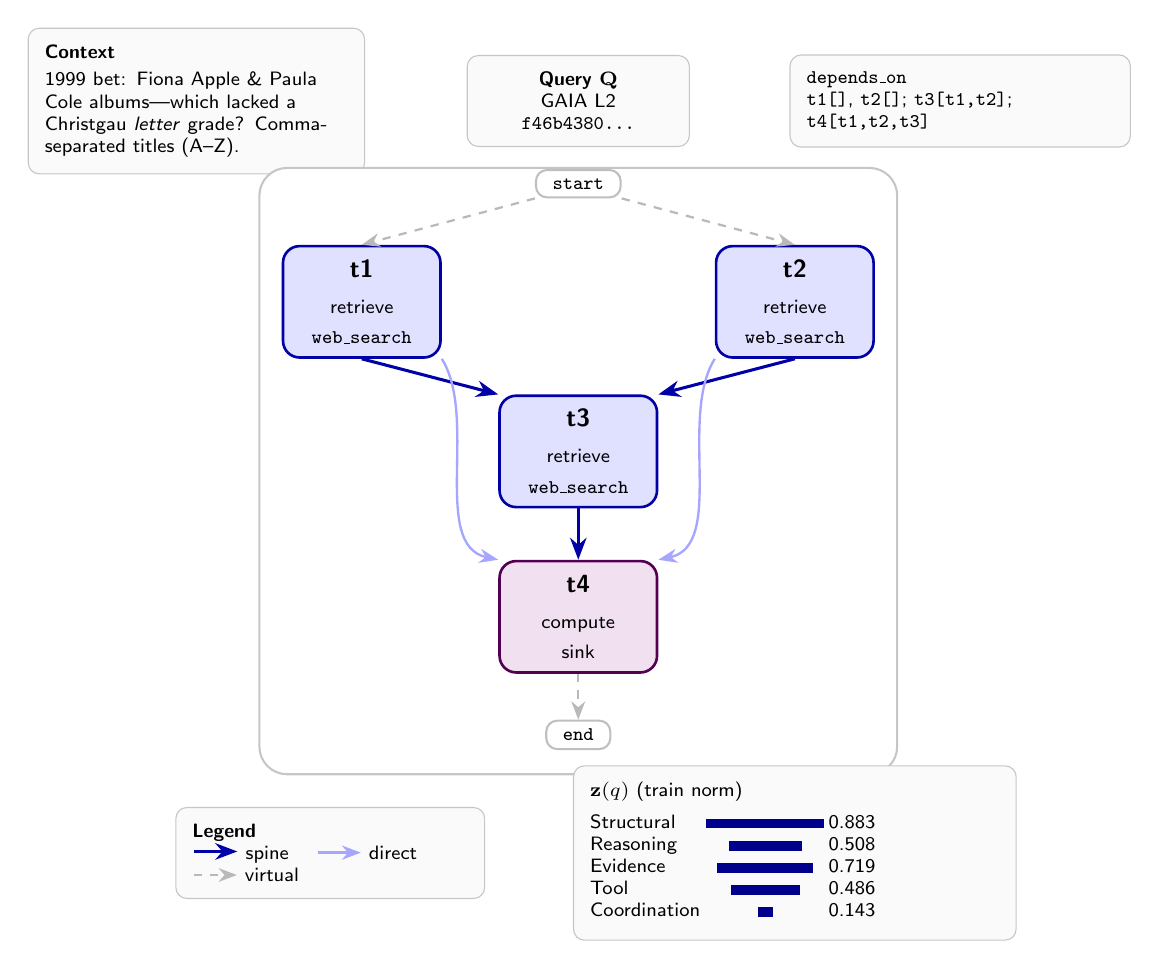
\begin{tikzpicture}[
    font=\small\sffamily,
    >=Stealth,
    panel/.style={
      draw=gray!45, rounded corners=4pt, fill=gray!4,
      inner sep=6pt, align=left, font=\scriptsize\sffamily,
    },
    st/.style={
      draw=#1!65!black, fill=#1!12, rounded corners=6pt,
      minimum width=2.0cm, minimum height=1.15cm, align=center,
      line width=0.95pt, inner sep=5pt,
    },
    virtnode/.style={
      draw=gray!50, fill=white, line width=0.75pt,
      rounded corners=4pt, font=\scriptsize\sffamily\ttfamily,
      inner xsep=6pt, inner ysep=3pt,
    },
    dep/.style={->, line width=1.1pt, draw=blue!65!black},
    depside/.style={->, line width=0.85pt, draw=blue!35},
    virtedge/.style={->, line width=0.8pt, draw=gray!55, dashed},
  ]
    % ===== Top metadata =====
    \node[panel, text width=3.85cm] (ctx) at (-4.85, 9.2) {%
      \textbf{Context}\\[2pt]
      1999 bet: Fiona Apple \& Paula Cole albums---which lacked a Christgau \emph{letter} grade? Comma-separated titles (A--Z).
    };
    \node[panel, text width=2.4cm, align=center] (qinfo) at (0, 9.2) {%
      \textbf{Query} $\mathbf{Q}$\\
      GAIA L2 \texttt{f46b4380\ldots}
    };
    \node[panel, text width=3.9cm] (edgebox) at (4.85, 9.2) {%
      \textbf{\texttt{depends\_on}}\\
      \texttt{t1[]}, \texttt{t2[]}; \texttt{t3[t1,t2]}; \texttt{t4[t1,t2,t3]}
    };

    % ===== DAG background (white, behind nodes) =====
    \fill[white, rounded corners=10pt] (-4.05, 0.65) rectangle (4.05, 8.35);
    \draw[gray!45, rounded corners=10pt, line width=0.75pt]
      (-4.05, 0.65) rectangle (4.05, 8.35);

    % ===== DAG nodes: start (top) -> end (bottom) =====
    \node[virtnode] (start) at (0, 8.15) {start};

    \node[st=blue] (t1) at (-2.75, 6.65) {%
      \textbf{t1}\\[2pt]
      {\scriptsize retrieve}\\
      {\scriptsize\texttt{web\_search}}};
    \node[st=blue] (t2) at (2.75, 6.65) {%
      \textbf{t2}\\[2pt]
      {\scriptsize retrieve}\\
      {\scriptsize\texttt{web\_search}}};

    \node[st=blue] (t3) at (0, 4.75) {%
      \textbf{t3}\\[2pt]
      {\scriptsize retrieve}\\
      {\scriptsize\texttt{web\_search}}};

    \node[st=violet] (t4) at (0, 2.65) {%
      \textbf{t4}\\[2pt]
      {\scriptsize compute}\\
      {\scriptsize sink}};

    \node[virtnode] (end) at (0, 1.15) {end};

    % ===== DAG edges (downward flow) =====
    \draw[virtedge] (start.south west) -- (t1.north);
    \draw[virtedge] (start.south east) -- (t2.north);
    \draw[dep] (t1.south) -- (t3.north west);
    \draw[dep] (t2.south) -- (t3.north east);
    \draw[dep] (t3.south) -- (t4.north);
    \draw[virtedge] (t4.south) -- (end.north);
    \draw[depside] (t1.south east) to[out=-58, in=168, looseness=0.85] (t4.north west);
    \draw[depside] (t2.south west) to[out=-122, in=12, looseness=0.85] (t4.north east);

    % ===== Bottom metadata =====
    \node[panel, text width=3.5cm] (leg) at (-3.15, -0.35) {%
      \textbf{Legend}\\
      \tikz{\draw[dep] (0,0) -- (0.55,0);} spine \quad
      \tikz{\draw[depside] (0,0) -- (0.55,0);} direct\\
      \tikz{\draw[virtedge] (0,0) -- (0.55,0);} virtual
    };
    \node[panel, text width=5.2cm, align=left] (zq) at (2.75, -0.35) {%
      \textbf{$\mathbf{z}(q)$} (train norm)\\[3pt]
      \begin{tabular}{@{}l@{\hspace{0.3em}}c@{\hspace{0.2em}}r@{}}
        Structural    & \textcolor{blue!55!black}{\rule{1.5cm}{0.12cm}} & 0.883 \\
        Reasoning     & \textcolor{blue!55!black}{\rule{0.92cm}{0.12cm}} & 0.508 \\
        Evidence      & \textcolor{blue!55!black}{\rule{1.22cm}{0.12cm}} & 0.719 \\
        Tool          & \textcolor{blue!55!black}{\rule{0.88cm}{0.12cm}} & 0.486 \\
        Coordination  & \textcolor{blue!55!black}{\rule{0.20cm}{0.12cm}} & 0.143 \\
      \end{tabular}
    };

  \end{tikzpicture}%
  }

  \caption{Worked GAIA example (eval \texttt{f46b4380-207e-4434-820b-f32ce04ae2a4}): procedure
    DAG $G_q$ (top \texttt{start} $\rightarrow$ bottom \texttt{end}) with parallel retrieves
    \texttt{t1}, \texttt{t2}, merge at \texttt{t3}, and fan-in sink \texttt{t4}
    (Table~\ref{tab:gaia-subtasks}). Curved edges are direct \texttt{depends\_on} links to the sink.
    Normalized $\mathbf{z}(q)$ in Table~\ref{tab:gaia-cq}.}
  \label{fig:gaia-dag-example}
\end{figure*}


The router then concatenates $\mathbf{z}(q)$ with $\psi(q)$ (PCA-16 embedding of the query
text) to form $\phi(q)$ for cost-soft HGBM routing.
This example illustrates how multi-hop GAIA queries with parallel evidence gathering and
merge nodes yield higher structural and evidence complexity than single-file linear plans.


\section{Hyperparameters and Reproducibility}
\label{app:hyperparameters}

\begin{table}[h]
  \centering
  \footnotesize
  \caption{Implementation details and hyperparameters (primary system).}
  \label{tab:hyperparams}
  \begin{tabular}{@{}ll@{}}
    \toprule
    Component & Setting \\
    \midrule
    \multicolumn{2}{@{}l}{\textit{Routing benchmark splits}} \\
    Train / validation / test queries & 808 / 100 / 100 \\
    \midrule
    \multicolumn{2}{@{}l}{\textit{QCE decomposition (Appendix~\ref{app:decompose-prompts})}} \\
    Procedure planner model & \texttt{gpt-4o-mini} \\
    Planner output & JSON subtask DAG $\rightarrow$ $G_q$ \\
    \midrule
    \multicolumn{2}{@{}l}{\textit{Representation (complexity--semantic)}} \\
    Planner complexity dimensions & 5 \\
    Semantic embedding (PCA) & 16 \\
    Total feature dimension & 21 \\
    \midrule
    \multicolumn{2}{@{}l}{\textit{Classifier and supervision}} \\
    Classifier & Gradient-boosted trees (HGBM) \\
    Training target & Cost-soft $p^\star$ (KL loss) \\
    Cost-soft temperature $\tau$ & 100 \\
    Utility-softmax $\tau$ (ablation; val-selected) & 0.05 \\
    \midrule
    \multicolumn{2}{@{}l}{\textit{Evaluation}} \\
    Utility weight $\lambda$ & 25 \\
    Selective gating threshold (transfer) & 0.5 \\
  \end{tabular}
\end{table}

\paragraph{Reproducibility.}
All benchmark splits, oracle outcomes, and feature representations are versioned and
released with the accompanying codebase.
Supplementary figures and per-dataset routing statistics are included in the supplementary
material.

\section{Additional Analyses}
\label{app:additional-analyses}

\paragraph{Routing policy analysis.}
Per-dataset strategy-selection distributions on executed benchmark workloads are provided
in the supplementary material.

\paragraph{Calibration.}
Figure~\ref{fig:calibration} shows reliability diagrams on the held-out test split of the
routing benchmark (generate with
\texttt{python -m research.analysis --split test} $\rightarrow$
\texttt{results/reports/router/test/reliability\_calibration.png}).

\begin{figure}[h]
  \centering
  \IfFileExists{results/reports/router/test/reliability_calibration.png}{%
    \includegraphics[width=0.75\linewidth]{results/reports/router/test/reliability_calibration.png}%
  }{%
    \IfFileExists{results/reports/router/val/reliability_calibration.png}{%
      \includegraphics[width=0.75\linewidth]{results/reports/router/val/reliability_calibration.png}%
    }{%
      \IfFileExists{results/reports/analysis/reliability_calibration.png}{%
        \includegraphics[width=0.75\linewidth]{results/reports/analysis/reliability_calibration.png}%
      }{%
        \fbox{\parbox[c][1in][c]{0.85\linewidth}{\centering\small
          Run \texttt{python -m research.analysis --split test}; expected at
          \texttt{results/reports/router/test/reliability\_calibration.png}.}}%
      }%
    }%
  }
  \caption{Router probability calibration (routing benchmark test split).}
  \label{fig:calibration}
\end{figure}

\paragraph{Cost--accuracy tradeoff.}
Figure~\ref{fig:cost-accuracy} compares cost--accuracy frontiers for routed and fixed
policies on the routing benchmark test split (same analysis run as above, or
\texttt{python -m research.figures} for
\texttt{results/reports/figures/fig3\_cost\_accuracy\_frontier.png}).

\begin{figure}[h]
  \centering
  \IfFileExists{results/reports/router/test/cost_vs_accuracy.png}{%
    \includegraphics[width=0.75\linewidth]{results/reports/router/test/cost_vs_accuracy.png}%
  }{%
    \IfFileExists{results/reports/analysis/cost_vs_accuracy.png}{%
      \includegraphics[width=0.75\linewidth]{results/reports/analysis/cost_vs_accuracy.png}%
    }{%
      \IfFileExists{results/reports/figures/fig3_cost_accuracy_frontier.png}{%
        \includegraphics[width=0.75\linewidth]{results/reports/figures/fig3_cost_accuracy_frontier.png}%
      }{%
        \fbox{\parbox[c][1in][c]{0.85\linewidth}{\centering\small
          Run \texttt{python -m research.analysis --split test}; expected at
          \texttt{results/reports/router/test/cost\_vs\_accuracy.png}.}}%
      }%
    }%
  }
  \caption{Cost--accuracy tradeoff comparing routed and fixed-strategy policies.}
  \label{fig:cost-accuracy}
\end{figure}

\paragraph{Embedding dimension sensitivity.}
We ablate PCA projection size ($8$, $16$, $32$, $64$ dimensions).
Dimension $16$ is used in all primary experiments; larger projections do not improve
held-out regret on the routing benchmark.

\section{Fixed-Strategy Baselines (Per-Agent EM)}
\label{app:fixed-agent-em}

\begin{table}[h]
  \centering
  \footnotesize
  \caption{Fixed-strategy exact match (\%) by workload.}
  \begin{tabular}{@{}lrrrrr@{}}
    \toprule
    Workload & raw & cot & react & multiagent \\
    \midrule
    GAIA & 4.2 & 6.1 & 26.1 & 13.3 \\
    HotpotQA & 39.5 & 36.5 & 69.0 & 32.0 \\
    MuSiQue & 2.5 & 2.5 & 36.5 & 25.5 \\
    MMLU & 48.5 & 53.0 & 59.0 & 46.5 \\
    MATH & 31.0 & 69.5 & 63.0 & 56.0 \\
    \bottomrule
  \end{tabular}
\end{table}

\section{Selective QCE}
\label{app:selective}

An optional selective gate routes queries with high embedding-only confidence without
invoking planner decomposition.
Validation-split regret and executed MMLU-Pro results for this variant are reported in the
supplementary material.

\section{Related Work (Extended)}
\label{app:related-extended}

Section~\ref{sec:related-work} discusses RouteLLM, LLM-Blender, and GraphRouter as the
primary literature baselines for this work.
Table~\ref{tab:related-mapping} summarizes how each system maps to components of our
experimental design.

\begin{table}[h]
  \centering
  \footnotesize
  \caption{Mapping from literature routing baselines to AAR experiments.}
  \label{tab:related-mapping}
  \begin{tabular}{@{}p{0.22\linewidth}p{0.34\linewidth}p{0.36\linewidth}@{}}
    \toprule
    Baseline & Core idea & AAR instantiation \\
    \midrule
    RouteLLM &
      Cost-aware strong/weak model routing &
      Utility $U_a=r_a-\lambda c_a$ and regret (§\ref{sec:experiments-setup}) \\
    LLM-Blender &
      Rank/fuse multiple viable model outputs &
      Cost-soft $p^\star$ over correct strategies (Table~\ref{tab:soft-target}) \\
    GraphRouter &
      Graph-structured query--candidate routing &
      Procedure-DAG complexity $\mathbf{z}(q)$ + embeddings (Table~\ref{tab:feature-regret}) \\
    \bottomrule
  \end{tabular}
\end{table}

RouteLLM~\citep{ong2025routellm}, RouterDC~\citep{chen2024routerdc}, and HybridLLM~\citep{ding2024hybridllm} learn query-conditioned \emph{model} selection under
cost constraints; LLM-Blender~\citep{jiang2023llmblender} operates post-hoc on multiple generations; GraphRouter~\citep{feng2025graphrouter} and
AgentRouter~\citep{zhang2025agentrouter} use entity- or affiliation-centric graphs with GNN routing.
We route among four heterogeneous \emph{agent pipelines} with tabular policies, procedure
graphs, and cost-soft labels restricted to correct strategies.
Direct head-to-head replication of published systems is limited by task mismatch (model/API
routing vs.\ tool-using agent strategies); our tables compare learned and heuristic routers
in the unified four-strategy setting above.

\section{Discussion and Analysis}
\label{app:discussion}

\paragraph{Main result.}
On the routing benchmark, among the evaluated factors cost-soft supervision yields the largest
observed regret reduction: agent regret falls from $0.361$ to $0.192$ relative to hard labels,
and executed exact match rises from 63\% to 82\% (Table~\ref{tab:hard-vs-soft}).
Under cost-soft supervision, the complexity--semantic representation yields the lowest total
regret ($0.198$) and outperforms both embedding-only and heuristic feature sets
(Table~\ref{tab:feature-regret}).
The best configuration combines both components; preserving multiple cost-weighted correct
strategies during training and enriching $\phi(q)$ with planner-derived structure together
improve cost-aware routing under the objective the router is trained to optimize.

\paragraph{Secondary result.}
Benchmark transfer is a secondary evaluation with mixed outcomes: the metric shifts to
executed exact match on heterogeneous public workloads without per-query oracle access
at inference.
The proposed router remains competitive (48.1\% pooled EM) but does not consistently
outperform a simpler heuristic router (50.3\%) or the strongest fixed strategy per family
(Table~\ref{tab:benchmark-transfer-em}); this should not be read as invalidating
routing-benchmark regret gains.
Held-out families (GAIA, MMLU-Pro) and distribution shift likely contribute; the framework
is most reliable where training and evaluation share oracle multi-strategy supervision.
Transfer nevertheless shows that the router does not collapse to a single static policy and
remains usable under full execution.

\paragraph{Oracle reference.}
\textbf{Best agent} performance in Table~\ref{tab:live-benchmark} should be read as an
oracle headroom reference, not as evidence that learned routing is near-optimal on every
workload.
Large gaps between proposed and best-agent exact match (e.g., on GAIA and HotpotQA) indicate
substantial room for improved routing or richer strategy pools, while the routing-benchmark
regret metric captures progress toward the cost-aware objective used during training.

Supplementary analyses---routing policy distributions across workloads, cost--accuracy
tradeoffs on oracle splits, and classifier calibration---are reported in
Appendix~\ref{app:additional-analyses}.


\end{document}
